\section{最短路径}
\label{sec:最短路径}
王国的故事还在继续。根据指挥官给出的遍历方法，信使无一疏漏地将大敌来犯的消息传遍了王国的每一座城池、每一座要塞。士兵和居民们纷纷武装起来，
布起防御系统，准备迎接那场即将到来的大战。

\subsection{迪杰斯特拉算法}
接下来，一位指挥官提出了这样一个问题：若某个据点有重兵来犯，从首都派出军队去该据点支援，走哪条路，能够最快到达？这种求解从某顶点到图中其他所有顶点
的最短路径的问题，后来被称为\term{单源最短路径}问题。

为了解决这个问题，指挥官们将王国建模成了一个无向带权图，边的权表示走此路径需要消耗的时间。如图\ref{fig:最短路径王国地图}所示。
\begin{wrapfigure}{l}{0.35\textwidth}
    \centering
    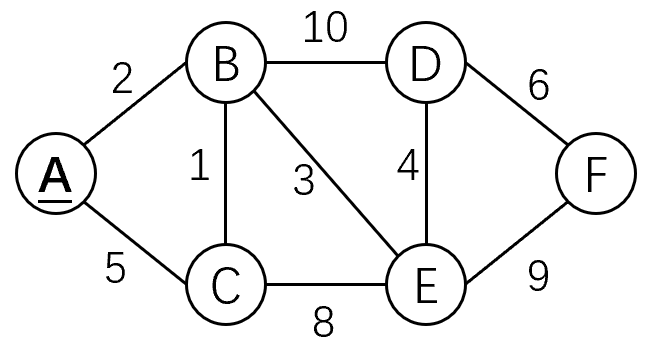
\includegraphics[width=0.35\textwidth]{assets/pics_and_ppts/ch5/10最短路径王国地图.png}
    \caption{}
    \label{fig:最短路径王国地图}
\end{wrapfigure}

假设A为首都，如何求A到F的最短路径？一位指挥官指出，最简单的做法就是把所有可能的路径都找出来，然后比较它们的长度。
这种做法通过DFS进行路径搜索即可实现，如{\color{red}\textbf{习题6第18题}}（
第\pageref{other:DFS求最短路径}页）所做的那样。但是，这种做法存在一个明显的问题：即使其中许多路径已经不可能成为最短路径，我们仍然要花费时间去搜索它们。
对图\ref{fig:最短路径王国地图}进行DFS路径搜索的\uwave{搜索树}如图\ref{fig:DFS搜索树}所示。可以看到每个叶节点即代表了一条路径的终点，
要么是找到了目标顶点，要么是非目标顶点的死路。

\begin{figure}[htbp]
    \centering
    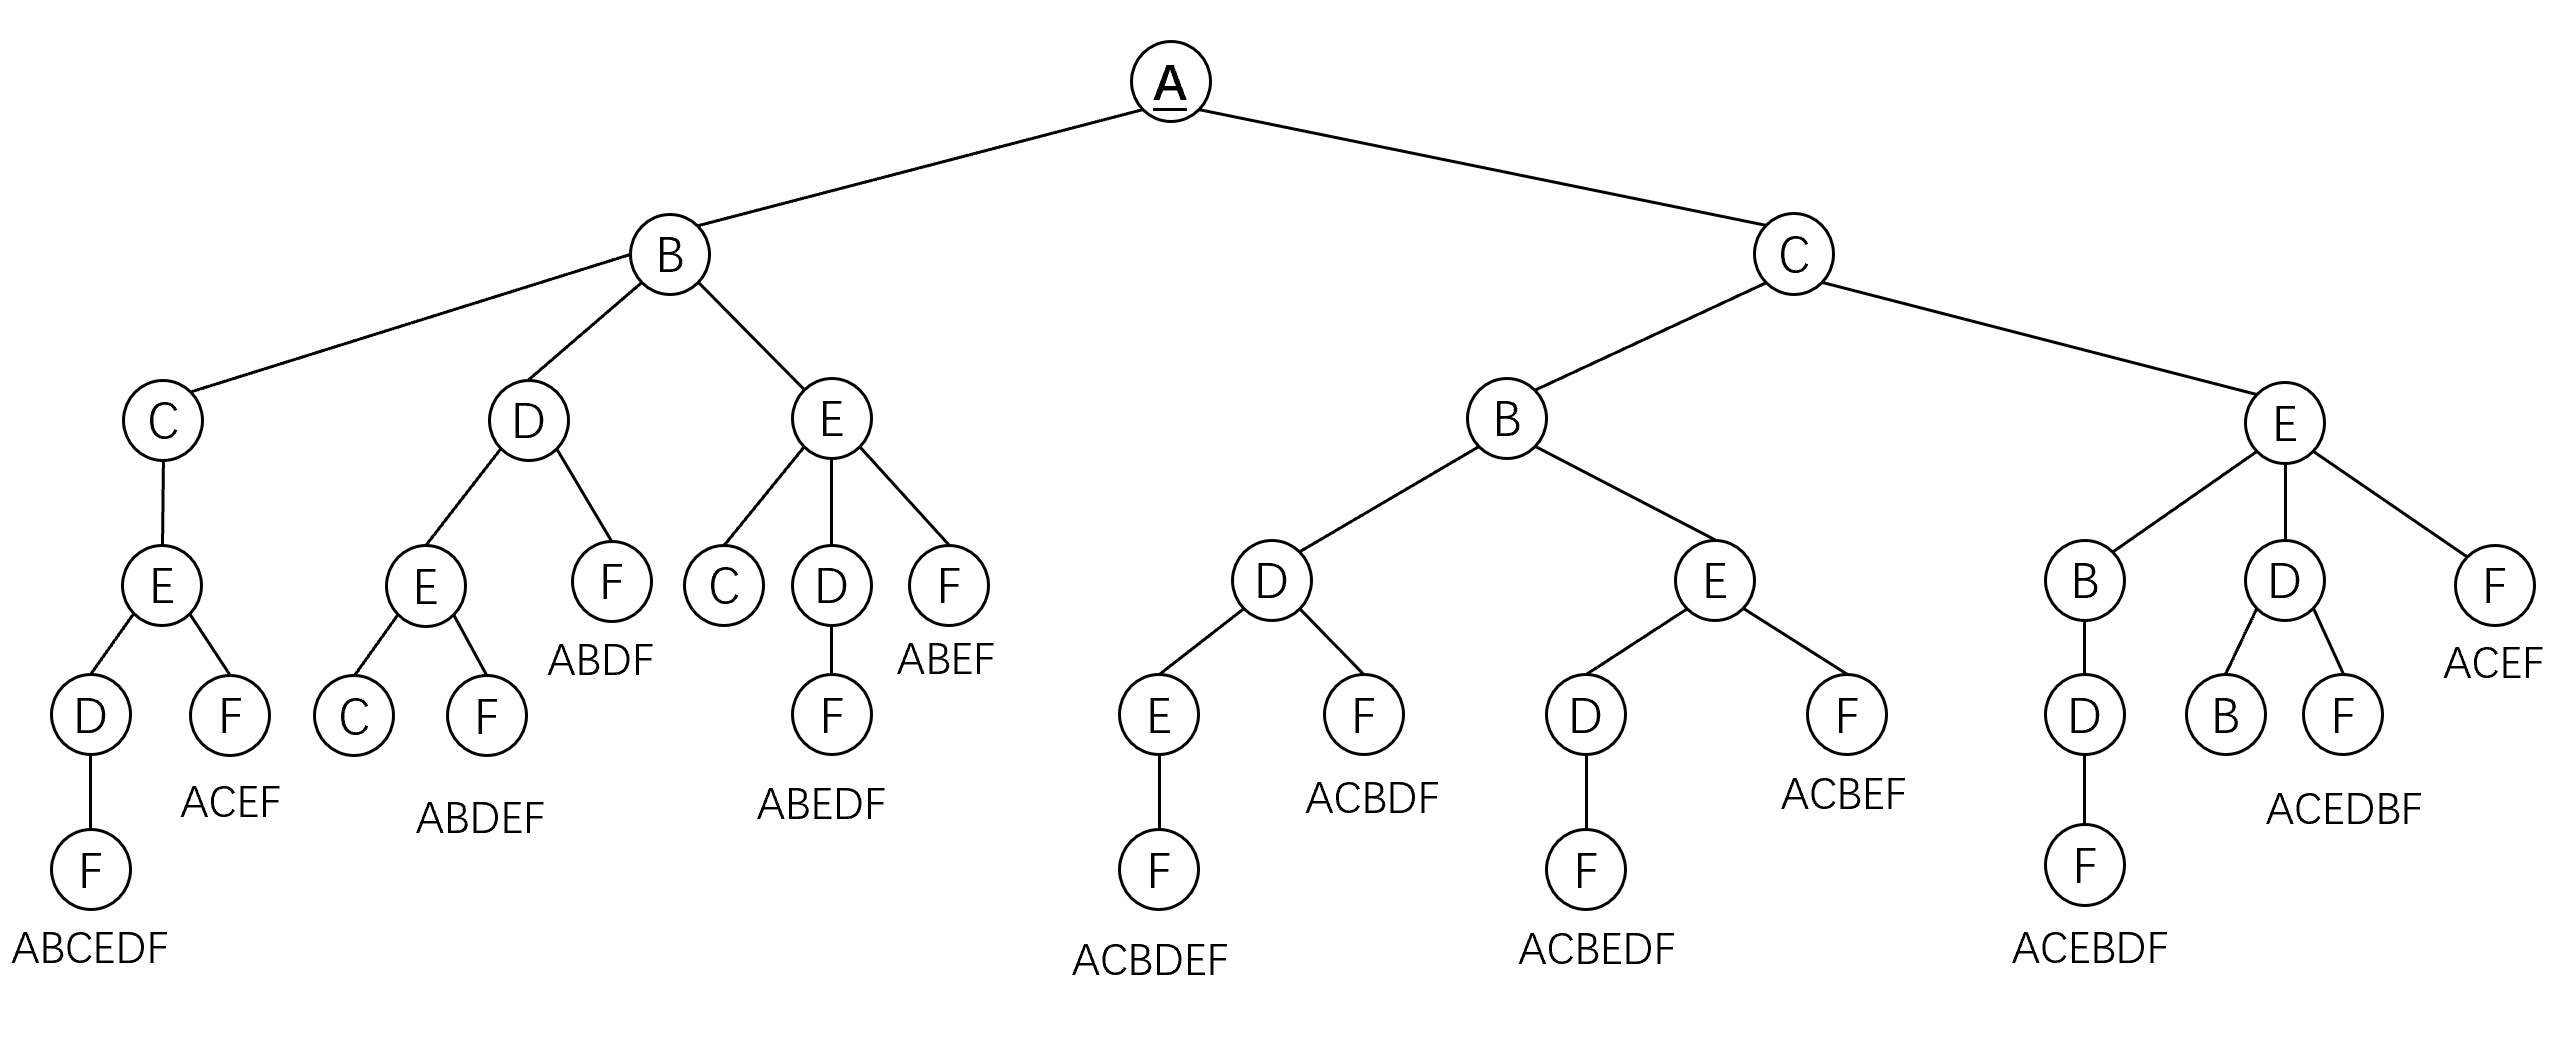
\includegraphics[width=1.05\textwidth]{assets/pics_and_ppts/ch5/11DFS搜索树.png}
    \caption{搜索树}
    \label{fig:DFS搜索树}
\end{figure}

当我们探索到一条可行的路径ABDF时，就已经知道最短路径
不可能大于4，于是ABEDF、ACBDEF等路径其实完全没有必要探索，即使使用\term{剪枝策略}（{\color{red}\textbf{见习题6第18题参考答案}}），
也要至少探索4个顶点再回头。DFS的穷举过程最差时间复杂度是$O(N!)$量级，对于稍微复杂的图，该算法绝对无法接受。况且如果需要求出A到所有顶点的最短路径，就需要
再重复如图\ref{fig:DFS搜索树}的搜索过程若干次。

\begin{notebox}{CoreLoop}
    \hspace{1.6em}我们暂时把思路拉回现实世界。
    
    \hspace{1.6em}执笔至此，笔者以为，接下来要介绍的迪杰斯特拉算法，大抵是本书中最令人惊叹、最具创造性的算法。
    我不想直接介绍迪杰斯特拉算法的过程与实现。我要尝试做一件事情：与你一起思考并探索迪杰斯特拉算法“诞生”的过程：当DFS绝对无法接受时，最短路径问题就摆在我们面前，
    我们将会有哪些思考和结论？以此过程，一方面加深大家对于算法的理解和记忆（而不是枯燥地记住这复杂的过程），另一方面，通过探索过程中的艰难到最后的柳岸花明，
    来体会算法开创者非凡的创造力，以此向艾兹赫尔·迪杰斯特拉（Edsger W. Dijkstra）---这位计算机领域的传奇人物致敬。

    \hspace{1.6em}\textbf{如你对此过程兴趣无多，请直接跳至\bookmarkref{bookmark:waypoint-8}{waypoint-8}处，这不会影响后面的旅途。}
\end{notebox}

首先，我们很容易想到这样一个想法：

\textbf{假设顶点$\boldsymbol{i}$正确的事实最短路径为$\boldsymbol{mind[i]}$}，那么，一定有：
\[
    mind[i] = min( mind[j_1] + cost(j_1, i), mind[j_2] + cost(j_2, i), ..., mind[j_n] + cost(j_n, i) )
\] 
其中，\(j_1, j_2, ..., j_n\)为$i$的所有邻接点，\(cost(j, i)\)表示顶点$j$到$i$的花费。
\begin{wrapfigure}{l}{0.30\textwidth}
    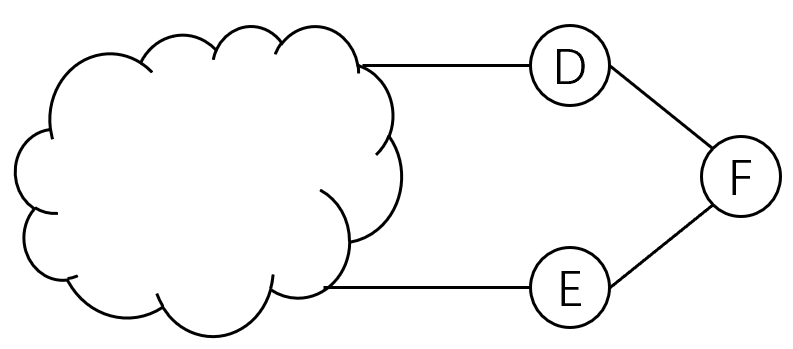
\includegraphics[width=0.30\textwidth]{assets/pics_and_ppts/ch5/13到达F必然经过D和E.png}
\end{wrapfigure}
例如如图\ref{fig:最短路径王国地图}中，要到达F，必然经过D或E，因此对于顶点F，一定有：
\[
    mind[F] = min( mind[D] + cost(D, F), mind[E] + cost(E, F) )
\]

也就是说，F的最短路径就是\Circled{1} A到D的最短路径 + D到F的花费 与 \Circled{2} A到E的最短路径 + E到F的花费 这二者之间更小的。
以上是\textbf{第一个事实}。那么只要确定了D、E的最短路径，F的最短路径也就确定了。

那么我们能不能先确定某些顶点的最短路径呢？\\

显然，顶点A到自身的花费（即$mind[A]$）一定是能确定的：就是0。这是因为路程花费时间不可能为负，所以A -> xxx -> A的花费一定更大。我们将这种
思想记为\textbf{“不绕弯思想”}。

同时，知道了mind[A]为0之后，对于顶点C，他有A、B、E三个邻接点，因此有：
\[
    mind[C] = min( mind[A] + cost(A, C), mind[B] + cost(B, C), mind[E] + cost(E, C) )
\]
其中的\(mind[A] + cost(A, C)\)这一项就能计算得出：\(0 + 5 = 5\)。于是我们可以记录下
来\textbf{当前已知的（并非全局的）C的最短路径$\boldsymbol{cur\_mind[C]} = 5$}，并在未来
某时刻确定了B、E的\(mind[B]\)和\(mind[E]\)时，若\(mind[B] + cost(B, C) < cur\_mind[C]\) 或 \(mind[E] + cost(E, C) < cur\_mind[C]\)，则可以用B或E
来更新\(cur\_mind[C]\)，这样最终得到的\(cur\_mind[C]\)一定是全局最短路径。于是我们顺着这个思路会自然地有这样的想法：\textbf{在确定了一个顶点的全局最短
路径mind[]时，要尝试更新其所有邻接点的最短路径，否则可能错过正确解。}

于是在知道了\(mind[A]\)之后我们更新所有A能到达的邻接点的“当前最短路径\(cur\_mind[]\)”，此时：
\begin{bulk}
    \begin{center}
        $cur\_mind[B] = 2$ \\
        $cur\_mind[C] = 5$
    \end{center}
\end{bulk}
而其他顶点暂未找到一条到达A的路径。如图\ref{fig:思考版迪杰斯特拉算法过程} a）所示，带下划线的数字表示该顶点当前已知的最短路径$cur\_mind[]$，
顶点有填充则表示该顶点的全局事实最短路径已经确定。
\begin{figure}[htbp]
    \centering
    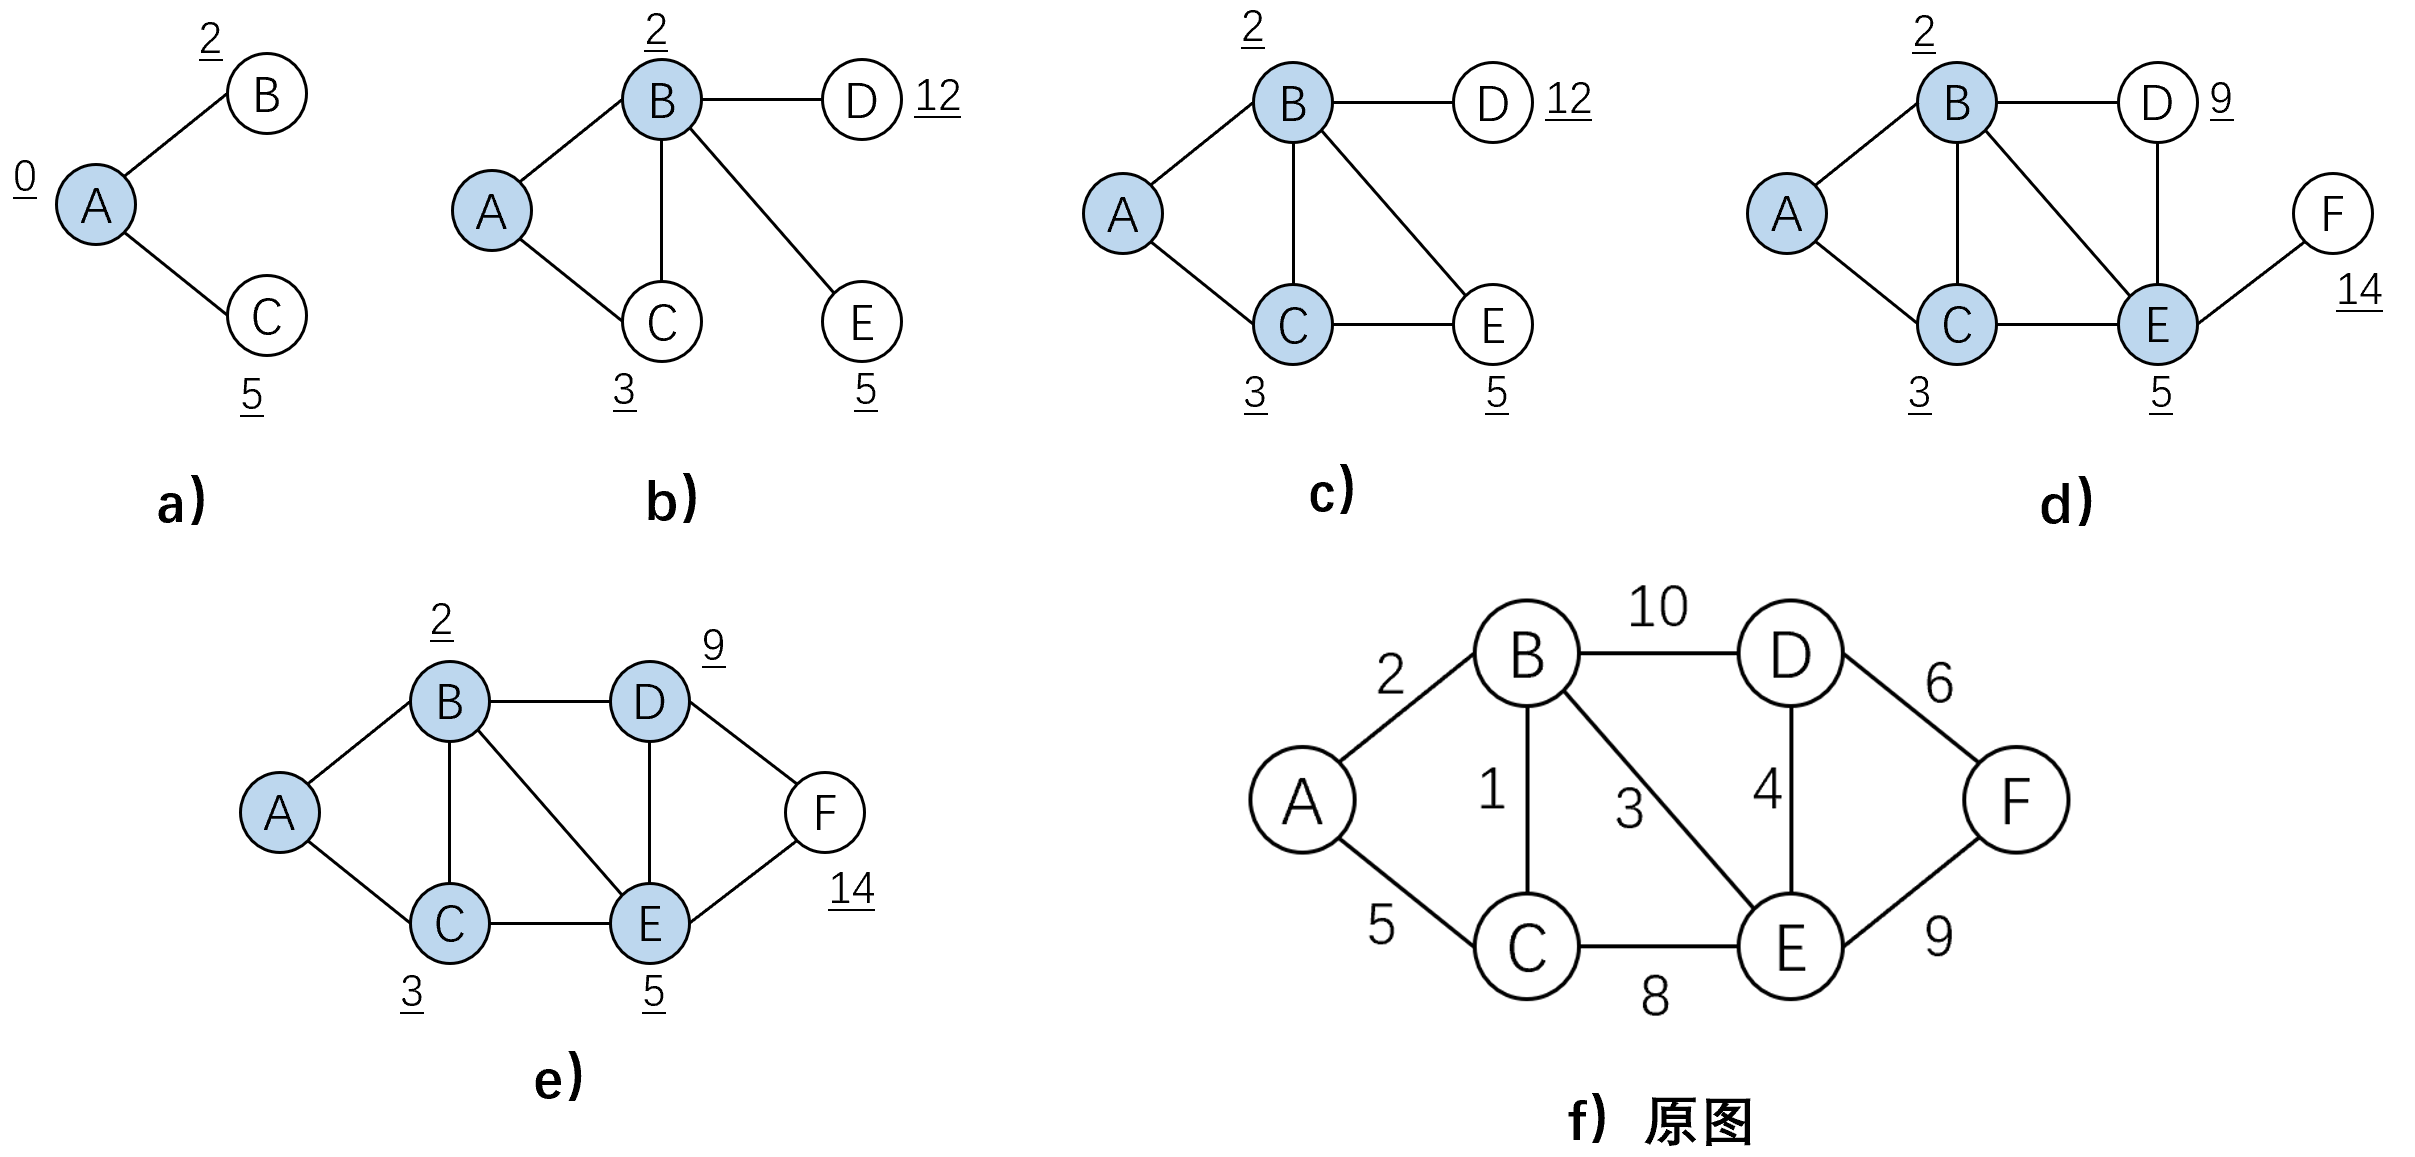
\includegraphics[width=0.99\textwidth]{assets/pics_and_ppts/ch5/12思考版迪杰斯特拉算法过程.png}
    \caption{}
    \label{fig:思考版迪杰斯特拉算法过程}
\end{figure}

我们会发现，此时\(cur\_mind[B] = 2\)一定是B的全局最短路径（因为B是所有A的邻接点中花费最小的那个，因此 A -> B 一定
比 A -> 非B 更短，结合“不绕弯思想”，B此时一定全局最短）。我们用集合$S$记录已经找到全局最短路径的顶点，此时
\[
    S = \{A, B\}
\]
如前所述，确定了$mind[B]$后，就可以更新与B邻接的C、D、E的当前已知最短路径$cur\_mind[]$信息：
\begin{bulk}
        $cur\_mind[C] = min(5, mind[B] + cost(B, C)) = min(5, 2+1) = 3$\\
        $cur\_mind[D] = mind[B]+cost(B,D) = 2 + 10 = 12$\\
        $cur\_mind[E] = 2 + 3 = 5$
\end{bulk}
如图\ref{fig:思考版迪杰斯特拉算法过程} b）所示。此时所有$cur\_mind[]$中，最小的就是$cur\_mind[C]$。根据“不绕弯思想”，显然此时C已知的当前最短一定
也是全局最短。可是，如何证明？接下来这部分便是迪杰斯特拉算法最为精彩也是最难理解的部分，还请听我慢慢道来。\\


如何证明当前已知的所有最短路径$cur\_mind[]$中最小的那个一定就是该顶点的全局最短路径？

如图\ref{fig:思考版迪杰斯特拉算法过程} b）所示，
由于A、B已确定全局最短路径，C还未确定，且所有可以到达C的路径中一定至少存在一个还未确定的顶点（至少有一个C还未确定），
我们假设\uline{存在}某条路径PATH到C的距离比$cur\_mind[C]$更短：
\begin{bulk}
    \begin{center}
        PATH: A -> xxx -> P -> X -> xxx -> C
    \end{center}
\end{bulk}
我们用X表示路径PATH中的第一个尚未确定全局最短路径的顶点，则它的前一个顶点P的全局最短路径一定已经确定。记这条路径PATH的长度为$L\_PATH$，
则我们实际上假设了
\[
    L\_PATH < cur\_mind[C]
\]
接下来，我们来一点一点证出该假设与事实相悖，从而推翻该假设。

由于P的全局最短路径已经确定，因此$cur\_mind[X]$一定已经由P点更新过，即此时一定有：
\[
    cur\_mind[X] <= mind[P] + cost(P, X)  \quad \text{\textbf{// 式（1）}}
\]
上不等式右边即是假设的那条路径PATH到X时的长度（A -> xxx -> P -> X的长度）。而由于图没有负权边，因此
\begin{bulk}
    A -> xxx -> P -> X
\end{bulk}
的长度一定小于等于
\begin{bulk}
    A -> xxx -> P -> X -> xxx -> C
\end{bulk}
的长度，即下式一定成立：
\[
    mind[P] + cost(P, X) <= L\_PATH    \quad \text{\textbf{// 式（2）}}
\]

于是整理式1式2，有：
\[
    cur\_mind[X] <= mind[P] + cost(P, X) <= L\_PATH   \quad \text{\textbf{// 式（3）}}
\]

而事实上C、X均是此时未确定最短路径的顶点，且C是所有$cur\_mind[]$中最小的那个，因此一定有：
\[
    cur\_mind[C] <= cur\_mind[X] \quad \text{\textbf{// 式（4）}}
\]
由式3、式4，得：
\[
    cur\_mind[C] <= cur\_mind[X] <= mind[P] + cost(P, X) <= L\_PATH
\]
这与我们假设的$L\_PATH < cur\_mind[C]$相悖，因此假设不成立，即不存在一条路径，其距离比当前已知的C的
最小距离$cur\_mind[C]$更小。

\textbf{由以上的过程，我们就证明了：当前已知的所有最短路径$cur\_mind[]$中最小的那个一定就是该顶点的全局最短路径。}\\

于是，接下来的思路就豁然开朗了：不断地选择当前已知的所有最短路径中最小的那个，作为该顶点的全局最短路径（已由上面的过程证明这是绝对正确的），接下来，
以该顶点为新的“中介”，去尝试更新其所有邻接点的$cur\_mind[]$，不断重复这个过程，直至所有顶点的全局最短路径都被确定。我们从C开始，看一遍接下来的过程。
\begin{figure}[htbp]
    \centering
    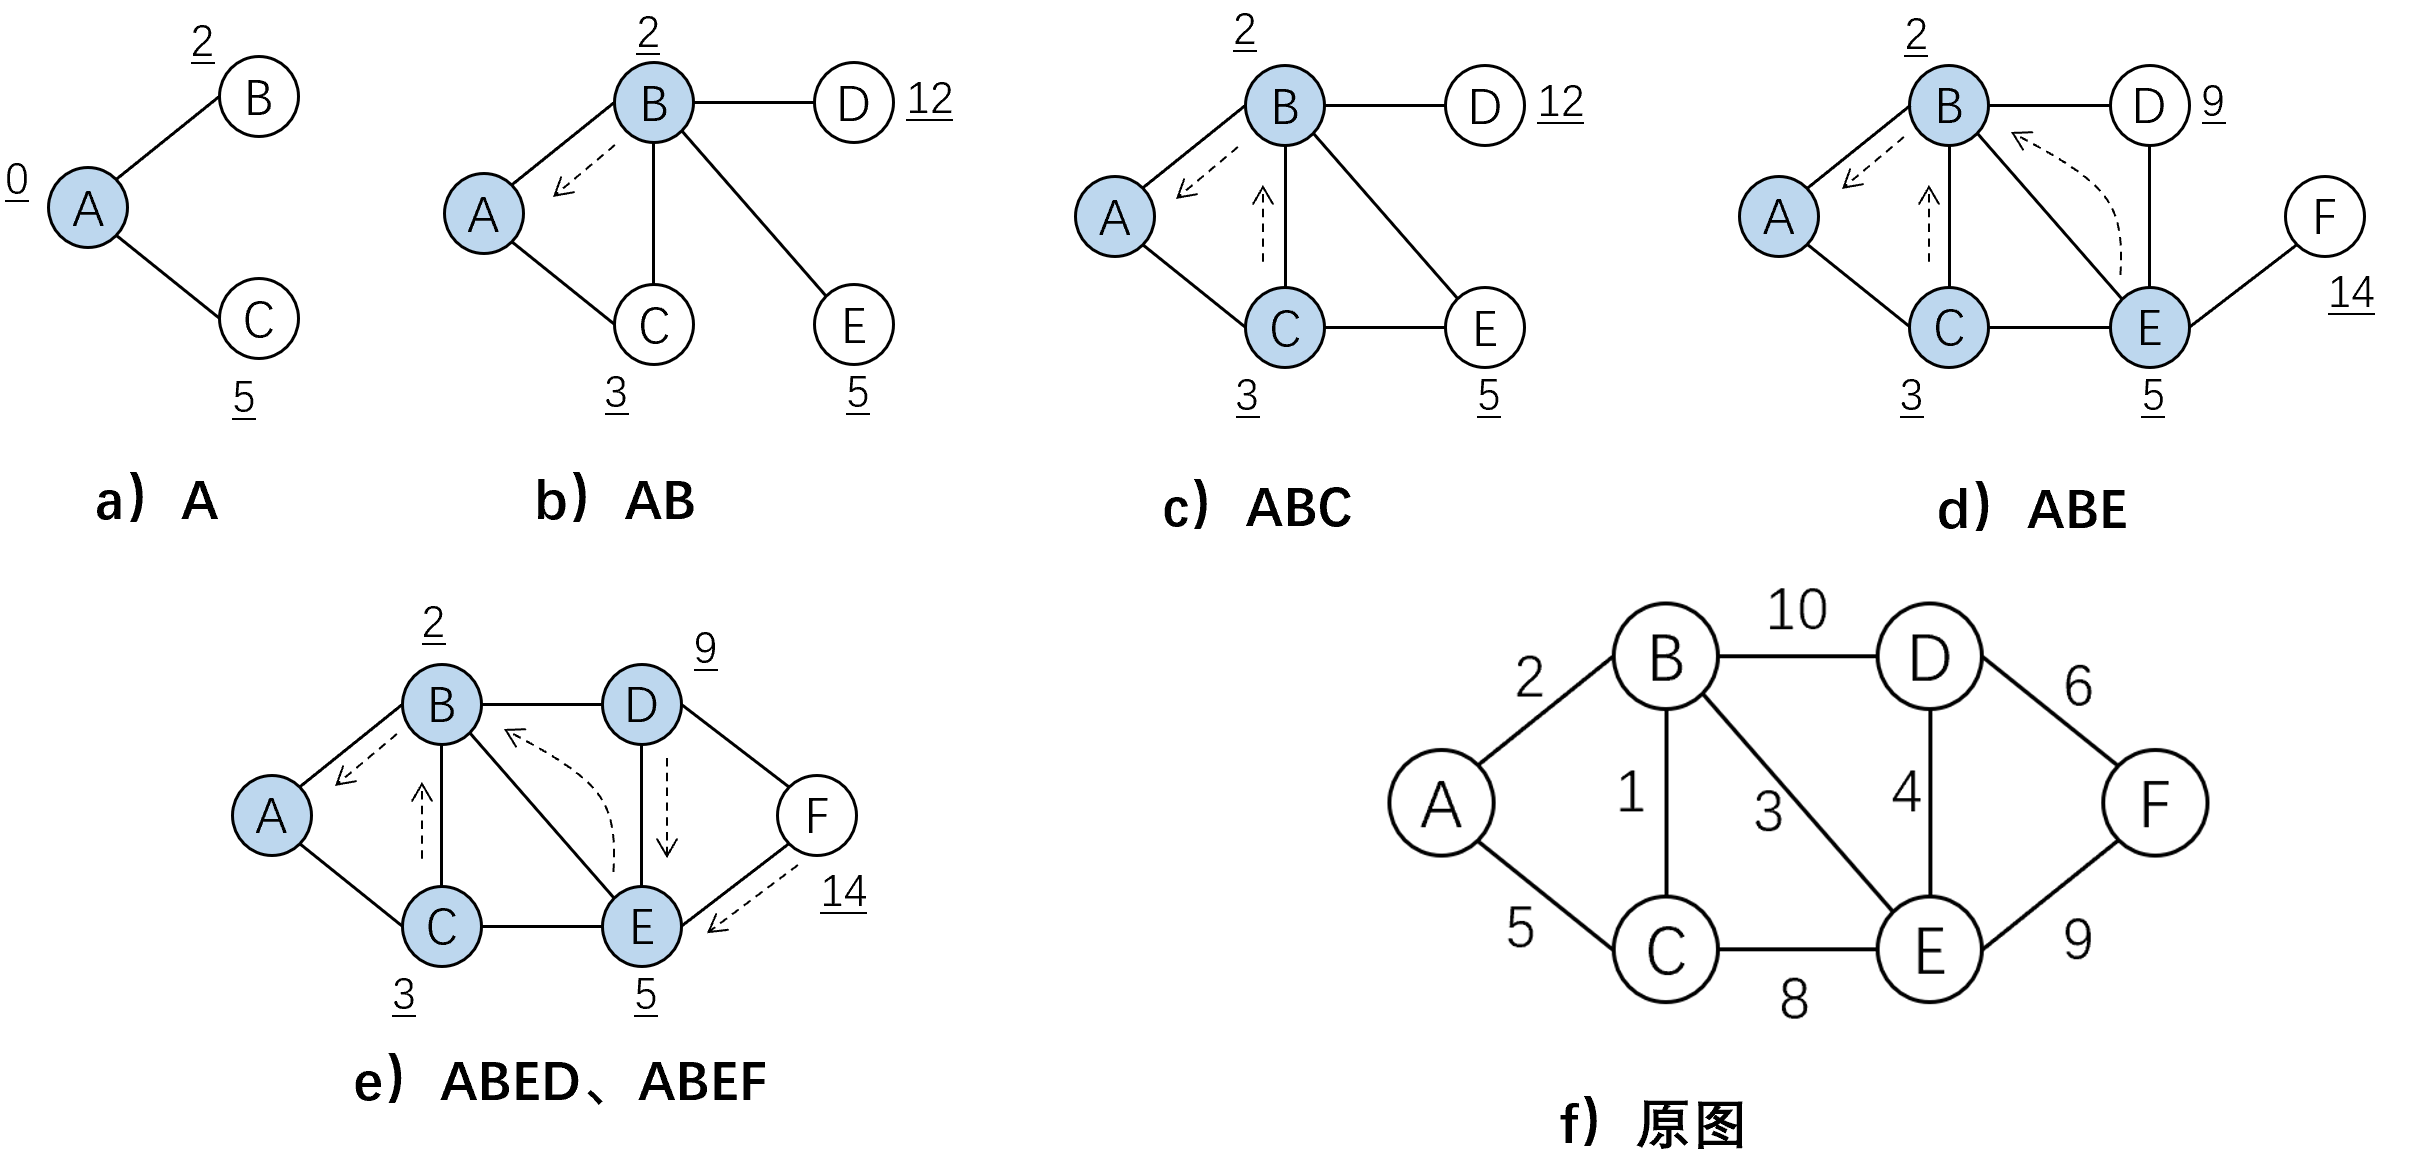
\includegraphics[width=0.99\textwidth]{assets/pics_and_ppts/ch5/14思考版迪杰斯特拉，带路径回溯.png}
    \caption{}
    \label{fig:思考版迪杰斯特拉，带路径回溯}
\end{figure}
如前所述，接下来将C的$cur\_mind[C]$作为C的全局最短，C也就成了“已求解”的顶点。所有已求解的顶点集合S就变成了：
\[
    S = \{A, B, C\}
\]
并且尝试更新$cur\_mind[E]$，但发现通过C到达E的距离：3 + 8 = 11不会比当前已知的：A -> B -> E（5）更短，因此$cur\_mind[E]$依然是5。如图
\ref{fig:思考版迪杰斯特拉，带路径回溯} c）所示。这一次我们在图中加入了路径回溯，记录每一个顶点最终的最短路径是由哪个顶点作为“中介”更新来的，如B
是由A更新来的，因此指向A，C是由B最终更新来的，因此指向B，以此方法记录最短路径本身（B是A -> B, C是A -> B -> C）。


继续从图中的 c）开始，此时$cur\_mind[D]=12$， $cur\_mind[E]=5$，最小的是$cur\_mind[E]$，因此E“已成功求解”，记$mind[E] = cur\_mind[E] = 5$，
并以E作为新的中介，计算：
\begin{bulk}
    $mind[E] + cost(E, D) = 5 + 4 = 9$，小于当前的$cur\_mind[D] = 12$，于是更新D\\
    $mind[E] + cost(E, F) = 5 + 9 = 14$，发现了一条新的到达F的路，所以更新F
\end{bulk}
更新后如图d）所示。最后一步，D作为“已成功求解”的顶点，并作为新的中介尝试更新F，但通过D到F不会更小，因此F的路径前驱依然是E，最终F也已成功求解，无其他顶点
了，如e）所示。

\begin{center}
    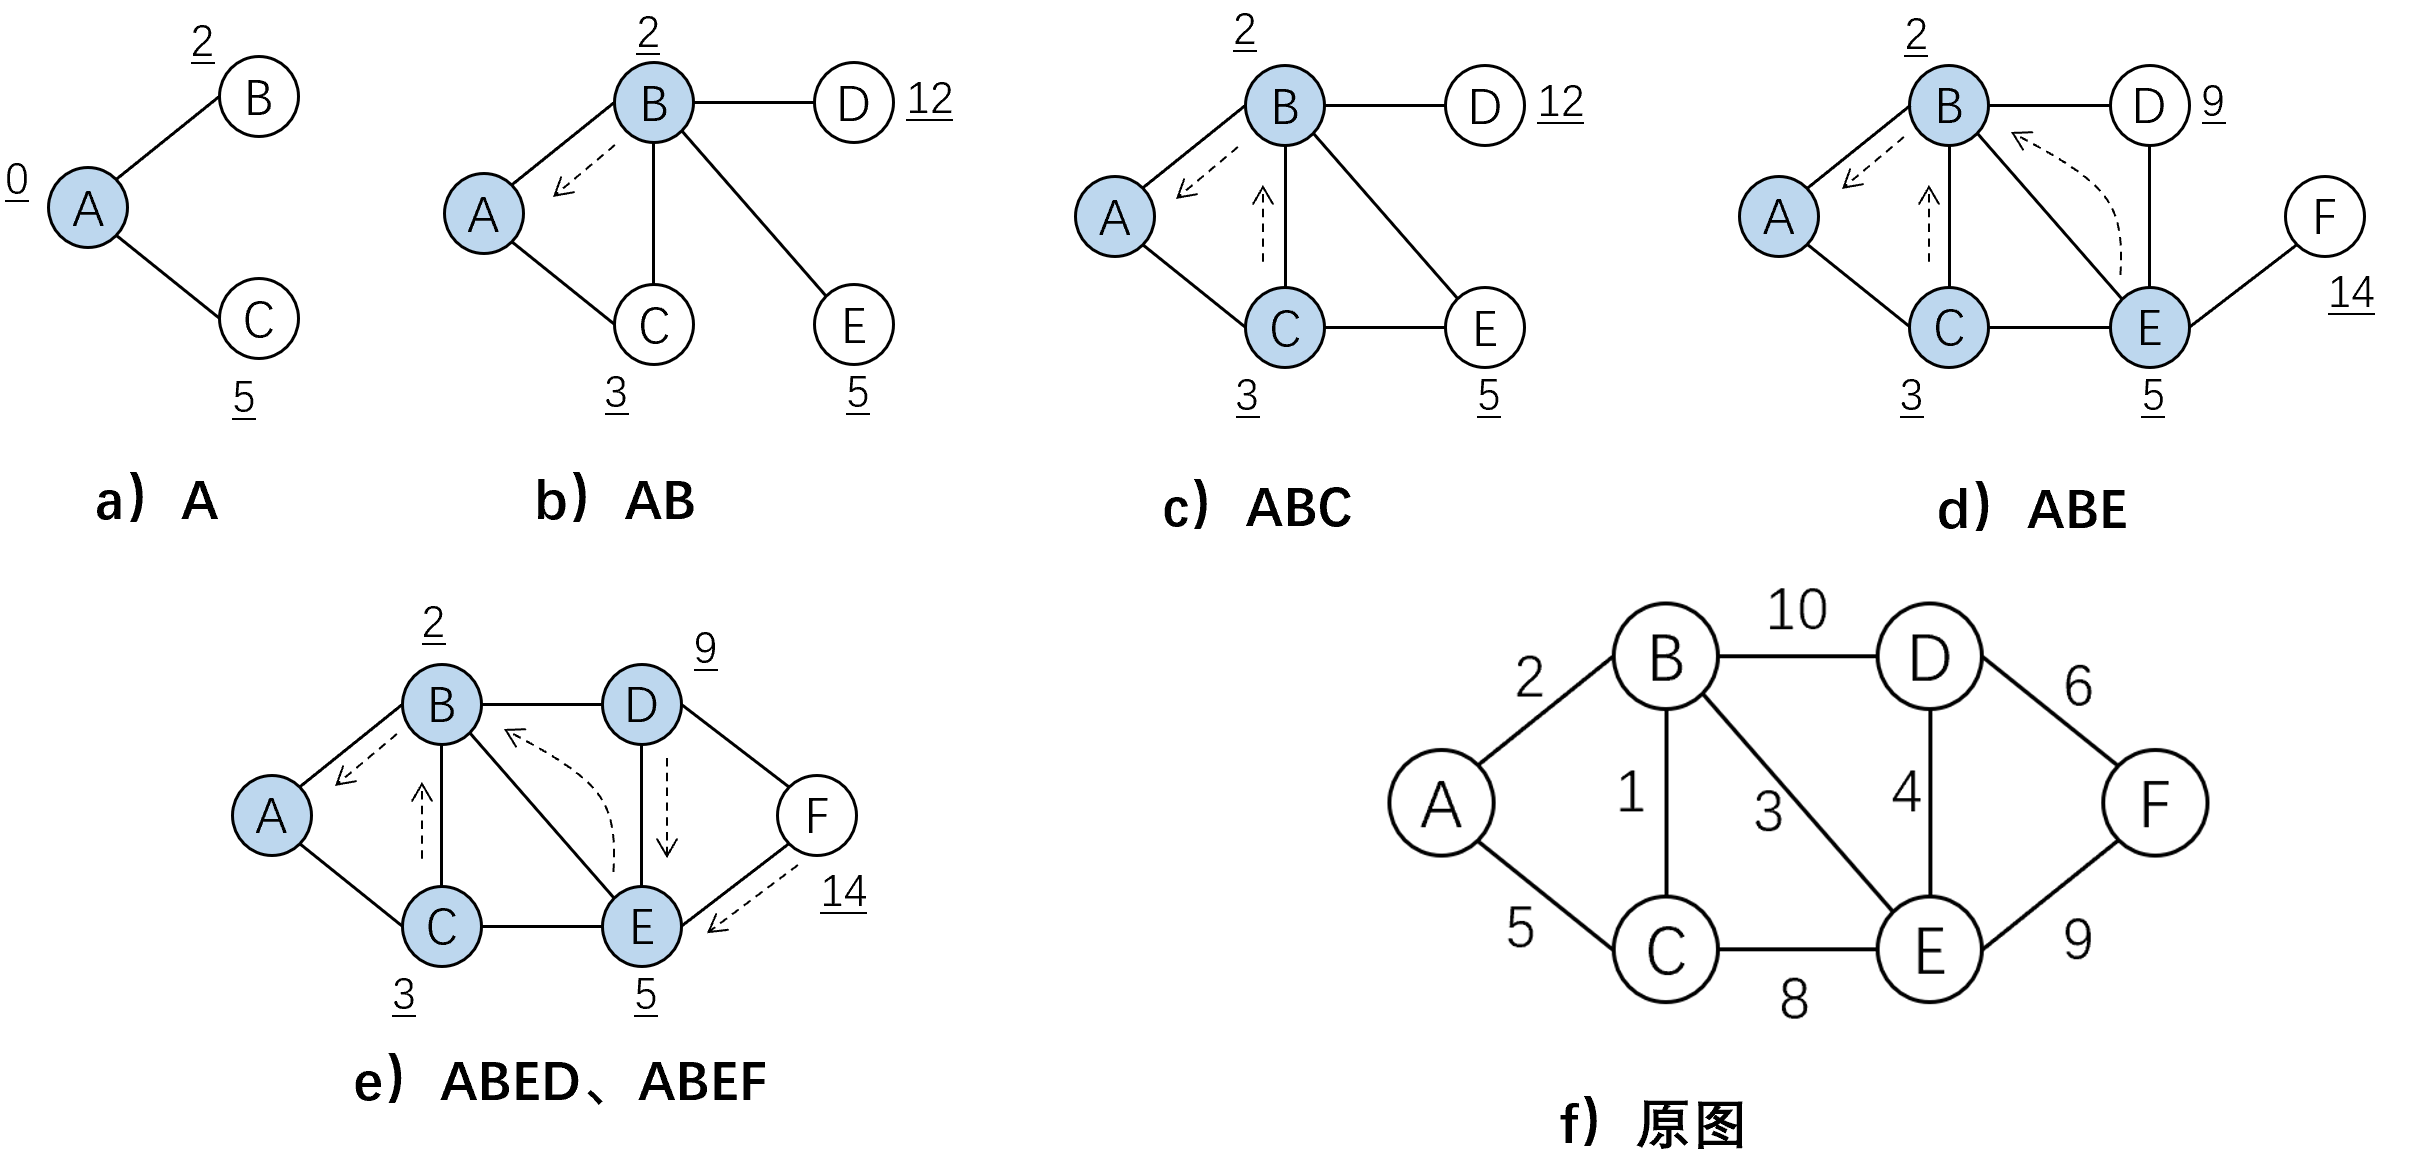
\includegraphics[width=0.99\textwidth]{assets/pics_and_ppts/ch5/14思考版迪杰斯特拉，带路径回溯.png}
\end{center}

至此，所有顶点到达A的最短路径均已求解，$cur\_mind[i]$中最终保存的就是顶点$i$到A的全局最短路径（事实最短路径），因为它一定已经经过了其所有邻接点的更新操作。

最后，需要注意我们以上讨论，都是基于一个假设：图中不存在负权边。通过上述过程也可以看得出来，若存在负边，“不绕弯思想”将不复存在，因此整个推理过程也将崩塌。
正是由于这样的道理，我们马上会看到，\textbf{迪杰斯特拉算法要求图中不存在从源点可达的负权边}。并且由以上思维过程我们知道，若图非连通，
迪杰斯特拉算法也可以得出哪些顶点从源点出发是不可达的。

\bookmark{bookmark:waypoint-8}{waypoint-8}
接下来我们正式介绍赫赫有名的迪杰斯特拉算法（Dijkstra算法）。我们先给出算法正确、完整的步骤，再由一个具体例子直观地感受一下。

\textbf{迪杰斯特拉算法}可用于求解单源最短路径问题。设图$G=(V,E)$有$N$个顶点，$cost(u, v)$为u到v的权值（路径的长度），我们记
$cur\_mind[i]$为顶点$i$当前已知的
最短路径长度，则求解起点$s$到其他任意顶点的最短路径的过程如下：

\begin{enumerate}
    \item 除起点s距离s为0（$cur\_mind[s]=0$）外，当前不知道任何其他顶点到s的最短路径，暂时认为所有顶点的最短路径都是正无穷+inf，将其他所有$cur\_mind[]$初始化为+inf。
    此时所有顶点均\textbf{未求解}。
    \item 从所有\textbf{未求解}顶点中，选出已知的最短路径长度$cur\_mind[]$最小的那个顶点v（第一次选的一定是s），
    该长度一定就是该顶点v到s的全局最短路径长度，于是v\textbf{“已求解”}。
    \item 以v为中介点，尝试更新所有v的邻接点的$cur\_mind[]$。具体来说，对于v的一条指向u的边，若$cur\_mind[v] + cost(v, u) < cur\_mind[u]$，说明经过v
    到u比之前已知的u到s的最短路径更短，所以将$cur\_mind[u]$ 更新为$cur\_mind[v] + cost(v, u)$。这一操作通常被称为\term{“松弛操作”}。
    \item 重复步骤 2 和步骤 3，直到所有可从起点 s 到达的顶点均已确定最短距离。
\end{enumerate}
\textbf{事实上迪杰斯特拉算法就是一个不断地“选点”、“更新”的过程}。我们设置一个数组Solved[]来标记哪些顶点已求解，哪些还未求解；并设立一个数组Pre[]标识每个顶点的路径
前驱，如Pre[1]值为0就表示顶点1的最短路径的上一步是从0走过来的。

我们以图\ref{fig:迪杰斯特拉算法过程演示图} f）所示的图为例来直观地感受一下迪杰斯特拉的过程。
\begin{figure}[htbp]
    \centering
    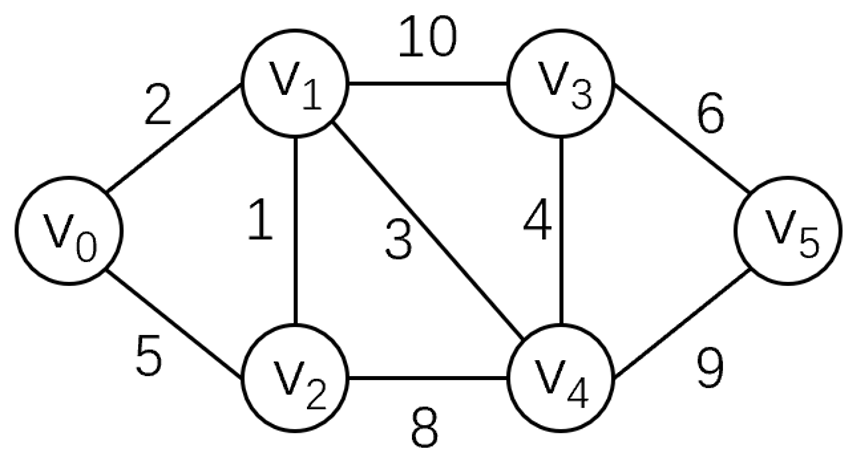
\includegraphics[width=0.40\textwidth]{assets/pics_and_ppts/ch5/15迪杰斯特拉算法过程演示.png}
    \caption{迪杰斯特拉算法过程演示图}
    \label{fig:迪杰斯特拉算法过程演示图}
\end{figure}

我们将$v_0$作为源点s，初始时，所有顶点均未求解，Solved[]为false，除源点s的$cur\_mind[0]=0$外，
所有其他顶点$cur\_mind[]$都是+inf，并且所有顶点的Pre[]均初始化为-1，表示尚未找到一条路径，暂无前驱，如表\ref{table:迪杰斯特拉算法过程演示}“初始”所示。
\begin{enumerate}
    \item
    \begin{minipage}[t]{0.65\linewidth}
        \vspace{0pt}
        从未求解顶点集合
        \{0,1,2,3,4,5\}
        中选择当前已知最短路径
        $cur\_mind[]$ 最小的顶点（0号顶点）。
        此时0号顶点的当前已知最短路径$cur\_mind[0]$一定也是全局最短路径，
        于是将$v_0$作为“已求解”顶点，
        Solved[0] 标记为 true。
        并且$v_0$就是起点，无前驱，
        $Pre[]$ 保持 -1 即可。然后以0号顶点为中介，尝试更新其邻接点$v_1$和$v_2$的$cur\_mind[]$:由于 $cur\_mind[v_0] + cost(v_0, v_1) = 0 + 2 = 2 < cur\_mind[v_1] = +inf$，
        因此将$cur\_mind[v_1]$更新为$cur\_mind[v_0] + cost(v_0, v_1)=2$，同理将$cur\_mind[v_2]$更新为0+5=5，由于$v_1$和$v_2$当前是由$v_0$更新来的，
        因此将Pre[1]和Pre[2]均设为0。
        
        如图a）及表\ref{table:迪杰斯特拉算法过程演示}步骤1所示。
    \end{minipage}
    \hfill
    \begin{minipage}[t]{0.30\linewidth}
        \vspace{0pt}
        \centering
        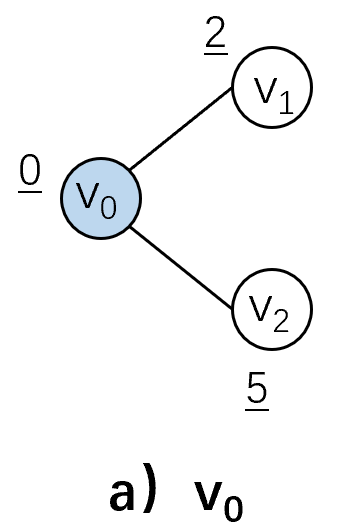
\includegraphics[width=0.67\linewidth]
        {assets/pics_and_ppts/ch5/16迪杰斯特拉过程a.png}
    \end{minipage}

    \item 
    \begin{minipage}[t]{0.65\linewidth}
        \vspace{0pt}
        从未求解顶点集合\{1,2,3,4,5\}中选择$cur\_mind[]$最小的顶点$v_1$，将该顶点的全局最短路径确定为2，并标记$v_1$的Solved[1]为true。然后
        以$v_1$为中介，$v_1$的邻接点有$v_2$、$v_3$、$v_4$，于是分别计算：$cur\_mind[v_1] + cost(v_1, v_2) = 3 < cur\_mind[v_2] = 5$，于是将
        $cur\_mind[v_2]$更新为3；$cur\_mind[v_1] + cost(v_1, v_3) = 12 < cur\_mind[v_3] = +inf$，于是将$cur\_mind[v_3]$更新为12，类似地，
        将$cur\_mind[v_4]$更新为5。并且$v_2$、$v_3$、$v_4$此时都是由$v_1$更新来的，因此将Pre[2]、Pre[3]、Pre[4]记为1。

        如图b）及表\ref{table:迪杰斯特拉算法过程演示}步骤2所示。
    \end{minipage}
    \hfill
    \begin{minipage}[t]{0.30\linewidth}
        \vspace{0pt}
        \centering
        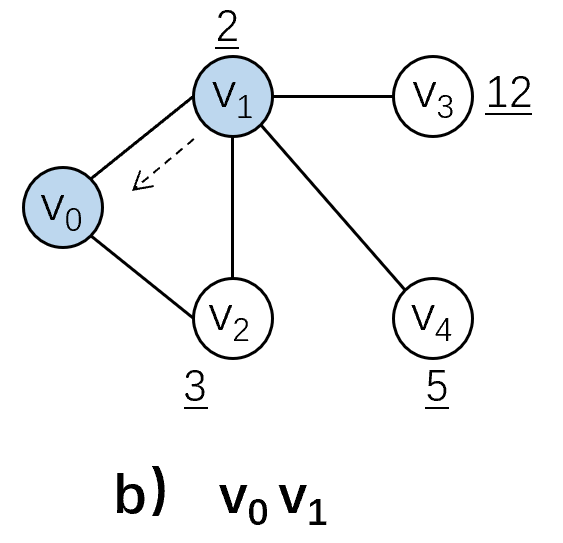
\includegraphics[width=0.88\linewidth]
        {assets/pics_and_ppts/ch5/17迪杰斯特拉过程b.png}
    \end{minipage}

    \item 
    \begin{minipage}[t]{0.65\linewidth}
        \vspace{0pt}
        从未求解顶点集合\{2,3,4,5\}中选择$cur\_mind[]$最小的顶点$v_2$，将Solved[2]标记为true，然后尝试更新$v_4$的$cur\_mind[4]$，但由于
        $cur\_mind[2] + cost(v_2, v_4) = 3 + 8 = 11 > cur\_mind[4] = 5$，因此无需更新。

        这一步其实只将顶点$v_2$标记为了“已求解”，如图c）及表\ref{table:迪杰斯特拉算法过程演示}步骤3所示。

    \end{minipage}
    \hfill
    \begin{minipage}[t]{0.30\linewidth}
        \vspace{0pt}
        \centering
        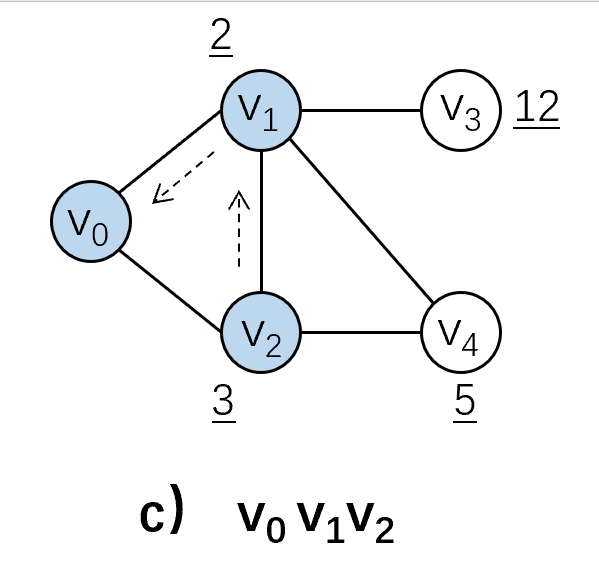
\includegraphics[width=0.90\linewidth]
        {assets/pics_and_ppts/ch5/18迪杰斯特拉过程c.png}
    \end{minipage}

    \item 
    \begin{minipage}[t]{0.65\linewidth}
        \vspace{0pt}
        从\{3,4,5\}中，选择顶点$v_4$，标记Solved[4]为true。并以$v_4$为中介，将$cur\_mind[3]$更新为9、Pre[3]更新为4；将$cur\_mind[5]$更新为5+9=14，将Pre[5]更新为4。

        如图d）及表\ref{table:迪杰斯特拉算法过程演示}步骤4所示。

    \end{minipage}
    \hfill
    \begin{minipage}[t]{0.30\linewidth}
        \vspace{0pt}
        \centering
        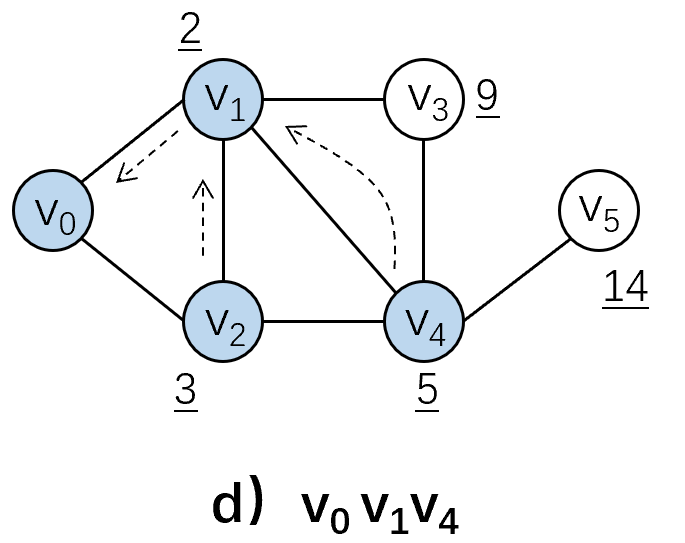
\includegraphics[width=0.99\linewidth]
        {assets/pics_and_ppts/ch5/19迪杰斯特拉过程d.png}
    \end{minipage}

    \item 
    \begin{minipage}[t]{0.65\linewidth}
        \vspace{0pt}
        从\{3,5\}中，选择顶点$v_3$，标记Solved[3]为true。以$v_3$为中介，发现$cur\_mind[3] + cost(3, 5) = 9+6 = 15 > cur\_mind[5] = 14$，因此无需更新。
        此时最后一个顶点$v_5$的最短路径显然也已经确定了，为14。

        如图e）及表\ref{table:迪杰斯特拉算法过程演示}步骤5所示。最后，我们将
        $v_5$标记为已求解顶点即可。

    \end{minipage}
    \hfill
    \begin{minipage}[t]{0.30\linewidth}
        \vspace{0pt}
        \centering
        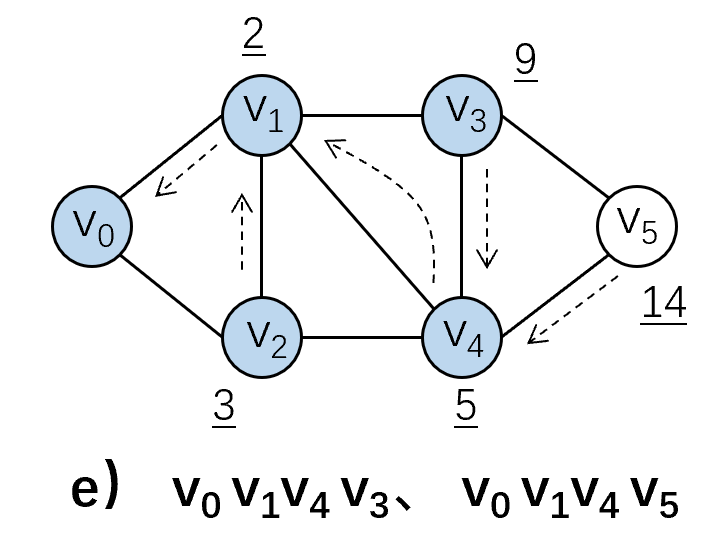
\includegraphics[width=0.99\linewidth]
        {assets/pics_and_ppts/ch5/20迪杰斯特拉过程e.png}
    \end{minipage}

    \item 将最后的顶点$v_5$标记为已求解。如表\ref{table:迪杰斯特拉算法过程演示}步骤6所示。

\end{enumerate}





\begin{table}[htbp]
    \centering
    \caption{迪杰斯特拉算法过程演示}
    \small
    \sffamily
    

    {
    \renewcommand{\arraystretch}{1.6}
    \setlength{\tabcolsep}{5pt}
    \setlength{\arrayrulewidth}{0.8pt}
    \arrayrulecolor{white}

    \begin{tabular}{
        |>{\columncolor{stepbg}\centering\arraybackslash}m{1.15cm}
        |>{\columncolor{fieldbg}\raggedright\arraybackslash}m{1.6cm}
        |*{7}{>{\columncolor{datablue}\color{white}\centering\arraybackslash}m{1.25cm}|}
    }
        \hline

        % 表头
        \multicolumn{2}{|c|}{
            \cellcolor{headblue}
            {\color{white}
            \diagbox[width=3.2cm,height=1.15cm,dir=NW]
            {\bfseries 步骤}
            {\bfseries 顶点}}
        }
        & \cellcolor{headblue}\textbf{0}
        & \cellcolor{headblue}\textbf{1}
        & \cellcolor{headblue}\textbf{2}
        & \cellcolor{headblue}\textbf{3}
        & \cellcolor{headblue}\textbf{4}
        & \cellcolor{headblue}\textbf{5}
        & \cellcolor{headblue}\textbf{剩余未求解顶点集合}
        \\
        \hline

        % 初始状态
        初始
        & \shortstack[l]{cur\_mind[]\\Pre[]\\Solved[]}
        & \shortstack[l]{0\\[0.23em]-1\\[0.23em]false} & \shortstack[l]{+inf\\[0.23em]-1\\[0.23em]false} & \shortstack[l]{+inf\\[0.23em]-1\\[0.23em]false} 
            & \shortstack[l]{+inf\\[0.23em]-1\\[0.23em]false}
        & \shortstack[l]{+inf\\[0.23em]-1\\[0.23em]false} & \shortstack[l]{+inf\\[0.23em]-1\\[0.23em]false} & \shortstack[l]{\{0,1,2,\\3,4,5\}}
        \\
        \hline

        % 第 1 步
        1
        & \shortstack[l]{cur\_mind[]\\Pre[]\\Solved[]}
        & \shortstack[l]{0\\[0.23em]-1\\[0.23em]\textbf{true}} & \shortstack[l]{\textbf{2}\\[0.23em]\textbf{0}\\[0.23em]false} & \shortstack[l]{\textbf{5}\\[0.23em]\textbf{0}\\[0.23em]false} 
            & \shortstack[l]{+inf\\[0.23em]-1\\[0.23em]false}
        & \shortstack[l]{+inf\\[0.23em]-1\\[0.23em]false} & \shortstack[l]{+inf\\[0.23em]-1\\[0.23em]false} & \shortstack[l]{\{1,2,\\3,4,5\}}
        \\
        \hline

        % 第 2 步
        2
        & \shortstack[l]{cur\_mind[]\\Pre[]\\Solved[]}
        & \shortstack[l]{0\\[0.23em]-1\\[0.23em]true} & \shortstack[l]{2\\[0.23em]0\\[0.23em]\textbf{true}} & \shortstack[l]{\textbf{3}\\[0.23em]\textbf{1}\\[0.23em]false} 
            & \shortstack[l]{\textbf{12}\\[0.23em]\textbf{1}\\[0.23em]false}
        & \shortstack[l]{\textbf{5}\\[0.23em]\textbf{1}\\[0.23em]false} & \shortstack[l]{+inf\\[0.23em]-1\\[0.23em]false} & \{2,3,4,5\}
        \\
        \hline

        % 第 3 步
        3
        & \shortstack[l]{cur\_mind[]\\Pre[]\\Solved[]}
        & \shortstack[l]{0\\[0.23em]-1\\[0.23em]true} & \shortstack[l]{2\\[0.23em]0\\[0.23em]true} & \shortstack[l]{3\\[0.23em]1\\[0.23em]\textbf{true}} 
            & \shortstack[l]{12\\[0.23em]1\\[0.23em]false}
        & \shortstack[l]{5\\[0.23em]1\\[0.23em]false} & \shortstack[l]{+inf\\[0.23em]-1\\[0.23em]false} & \{3,4,5\}
        \\
        \hline

        % 第 4 步
        4
        & \shortstack[l]{cur\_mind[]\\Pre[]\\Solved[]}
        & \shortstack[l]{0\\[0.23em]-1\\[0.23em]true} & \shortstack[l]{2\\[0.23em]0\\[0.23em]true} & \shortstack[l]{3\\[0.23em]1\\[0.23em]true} 
            & \shortstack[l]{\textbf{9}\\[0.23em]\textbf{4}\\[0.23em]false}
        & \shortstack[l]{5\\[0.23em]1\\[0.23em]\textbf{true}} & \shortstack[l]{\textbf{14}\\[0.23em]\textbf{4}\\[0.23em]false} & \{3,5\}
        \\
        \hline

        % 第 5 步
        5
        & \shortstack[l]{cur\_mind[]\\Pre[]\\Solved[]}
        & \shortstack[l]{0\\[0.23em]-1\\[0.23em]true} & \shortstack[l]{2\\[0.23em]0\\[0.23em]true} & \shortstack[l]{3\\[0.23em]1\\[0.23em]true} 
            & \shortstack[l]{9\\[0.23em]4\\[0.23em]\textbf{true}}
        & \shortstack[l]{5\\[0.23em]1\\[0.23em]true} & \shortstack[l]{14\\[0.23em]4\\[0.23em]false} & \{5\}
        \\
        \hline

        % 第 6 步
        6
        & \shortstack[l]{cur\_mind[]\\Pre[]\\Solved[]}
        & \shortstack[l]{0\\[0.23em]-1\\[0.23em]true} & \shortstack[l]{2\\[0.23em]0\\[0.23em]true} & \shortstack[l]{3\\[0.23em]1\\[0.23em]true} 
            & \shortstack[l]{9\\[0.23em]4\\[0.23em]true}
        & \shortstack[l]{5\\[0.23em]1\\[0.23em]true} & \shortstack[l]{14\\[0.23em]4\\[0.23em]\textbf{true}} & \{\;\}
        \\
        \hline

    \end{tabular}
    }
    \label{table:迪杰斯特拉算法过程演示}
\end{table}

% 恢复表格样式
\arrayrulecolor{black}
\setlength{\arrayrulewidth}{0.5pt}

可以看到，“选点”就是每次从尚未求解的集合中，“选”出一个当前已知最短路径$cur\_mind[]$最小的顶点v，作为“已求解顶点”，并用它尝试“更新”其所有邻接点的
最短路径$cur\_mind[]$。每次能确定一个顶点的全局最短路径，重复$N$次操作（其实$N-1$次即可），即可求解所有顶点的全局最短路径，最终$cur\_mind[]$
中保存的就是各个顶点的全局最短路径的长度，而各顶点的最短路径是什么，顺着Pre[]数组一路向前即可。如$v_5$到$v_0$的最短路径就是
\begin{bulk}
    5 -> Pre[5] = 4 -> Pre[4] = 1 -> Pre[1] = 0，即 5 -> 4 -> 1 -> 0    
\end{bulk}
这就是赫赫有名的迪杰斯特拉算法。迪杰斯特拉算法可以求解出从源点s到各个与之连通的顶点之间的最短路径，同时也可以确定哪些顶点与s是不连通的。但迪杰斯特拉算法要求
图中不存在从源点出发可达的负权边，\textbf{若图不满足这一条件，迪杰斯特拉算法将失效}。

迪杰斯特拉算法需要$N$次“选点”、“更新”操作，更新时需要找到该顶点的所有邻接点，而对于邻接矩阵和邻接表存储的图，找邻接点的时间复杂度有所区别，因此，迪杰斯特拉
算法的时间复杂度与图的存储方式有关，下面我们就看看两种存储方式下，迪杰斯特拉算法如何实现。

\minisection{1.迪杰斯特拉算法实现（邻接矩阵版）}
有了前面的思路，我们可以很轻松地写出迪杰斯特拉算法的代码。唯一需要注意的就是需要正确处理图中存在顶点不可达的情况，详请参见如下代码及注释。

\begin{cppcode}
    int Matrix[N][N];   // 邻接矩阵，存放边权，若边不存在用-1表示
    bool Solved[N];     // 已初始化为false
    int Pre[N];         // 已初始化为-1
    int cur_mind[N];    // 已初始化为 +inf。
    const int inf = 0x3fffffff; // +inf
    // 求解以s为源点的单源最短路径
    void Dijkstra(int s) {
        cur_mind[s] = 0;
        // 该层循环用于执行N次“选点”、“更新”的操作
        for(int i=0; i<N; i++) {
            // 选出未求解的顶点中，cur_mind[]最小的顶点v
            int min_cur_mind = inf;
            int v = -1;
            for(int j=0; j<N; j++) {
                if(Solved[j] == false && cur_mind[j] < min_cur_mind) {
                    min_cur_mind = cur_mind[j];
                    v = j;
                }
            }

            /* 这里是为了处理图中存在顶点不可达的情况。
             若存在顶点不可达，则将可达顶点全选完之后，
             接下来一定会“选不到顶点”，所以若没选到顶点，
             则v的值是无意义的，不应执行后面的代码。*/
            if(v == -1) {
                break;
            }
            
            Solved[v] = true;
            // 以v为中介，尝试更新其所有邻接点
            for(int u=0; u<N; u++) {
                // v到u有路径并且u的全局最短还未确定 不判断Solved[u] == false性能稍差一点，但影响不大。
                if(Matrix[v][u] != -1 && Solved[u] == false) {    
                    if(cur_mind[v] + Matrix[v][u] < cur_mind[u]) {
                        cur_mind[u] = cur_mind[v] + Matrix[v][u];
                        Pre[u] = v;
                    }
                }
            } 
        } 
    }
    
\end{cppcode}
对于以上邻接矩阵版的代码，需要$N$次“选点”、“更新”操作，外层循环时间为$O(N)$，每次选点时遍历一遍cur\_mind[]数组的时间是$O(N)$，更新时需要找到该顶点的所有邻接点，
时间是$O(N)$，整体的时间复杂度为$O(N^2)$。空间方面，需要额外引入Pre[]、Solved[]、cur\_mind[]三个数组，空间复杂度为$O(N)$。

注意：邻接矩阵是存储图本身所需要的空间，不属于迪杰斯特拉算法带来的空间开销，不能算在算法的空间复杂度中。

\minisection{2.迪杰斯特拉算法实现（邻接表版）}
邻接表版仅在获取顶点的邻接点信息时代码有所不同。邻接表版代码如下所示。
\begin{cppcodeHighlight}[1-5,30-36]
    struct AdjEdge {
        int u;      // 邻接点的编号
        int weight; // 边权
    };
    vector<AdjEdge> AdjList[N];    // 邻接表
    bool Solved[N];     // 已初始化为false
    int Pre[N];         // 已初始化为-1
    int cur_mind[N];    // 已初始化为 +inf。
    const int inf = 0x3fffffff; // +inf
    // 求解以s为源点的单源最短路径
    void Dijkstra(int s) {
        cur_mind[s] = 0;
        for(int i=0; i<N; i++) {
            // 选出未求解的顶点中，cur_mind[]最小的顶点v
            int min_cur_mind = inf;
            int v = -1;
            for(int j=0; j<N; j++) {
                if(Solved[j] == false && cur_mind[j] < min_cur_mind) {
                    min_cur_mind = cur_mind[j];
                    v = j;
                }
            }

            if(v == -1) {
                break;
            }
            
            Solved[v] = true;
            // 以v为中介，尝试更新其所有邻接点
            for(int j=0; j<AdjList[v].size(); j++) {
                int u = AdjList[v][j].u;  // 与v邻接的顶点u
                if(cur_mind[v] + AdjList[v][j].weight < cur_mind[u]) {
                    cur_mind[u] = cur_mind[v] + AdjList[v][j].weight;
                    Pre[u] = v;
                }
            }
        } 
    }
\end{cppcodeHighlight}
对于以上邻接表版的代码，外层循环时间同样为$O(N)$，每次选点时遍历一遍cur\_mind[]数组的时间同样是$O(N)$，而更新时找到该顶点的所有邻接点的操作
实际上与外层循环无关，是对整个图来说需要进行约$M$次，$M$为图的边数。因此邻接表版时间复杂度为$O(N^2+M)$。

空间方面，与邻接矩阵版本类似，同样是需要额外引入Pre[]、Solved[]、cur\_mind[]三个数组，空间复杂度为$O(N)$。

请注意，上面的代码中，每次寻找当前cur\_mind[]最小的顶点时，我们是遍历一遍数组，为O(N)的时间。事实上，可以使用前面介绍过的数据结构---\textbf{堆}
（C++中的priority\_queue）来完成，每次以O(1)时间
即可返回最小的元素。若图采用邻接表实现，这种堆优化的迪杰斯特拉算法的\textbf{最坏}时间复杂度可以达到$O((N+M)logN)$。由于priority\_queue在此处的使用涉及
稍复杂的C++原理，因此不在此处给出代码，感兴趣的同学可以自己尝试写出。



\subsection{Bellman-Ford算法}
几乎在迪杰斯特拉算法诞生的同期，也诞生了另外一个求解单源最短路径的算法：Bellman-Ford 算法。它与 Dijkstra 算法有一个重要区别：只要从源
点出发能够到达的范围内不存在负权\uline{环}，Bellman-Ford 算法就能够正确求得单源最短路径，即使图中存在负权边也没有问题。\\

Bellman-Ford算法的核心思想是：反复对图中的\uline{所有边}进行松弛操作。具体来说，假设图中有$N$个顶点$M$条边，源点为s，与迪杰斯特拉算法类似，定义：
cur\_mind[v]为当前已知的从s到v的最短路径长度，初始化cur\_mind[s]为0，其他顶点的cur\_mind[]均为正无穷。

然后，对图中的每一条边$(u, v)$ 进行松弛操作：
\[
    dist[v]=\min(dist[v], dist[u] + cost(u,v))
\]
其中，\(cost(u,v)\) 表示边 \((u,v)\) 的权值（路径长度）。对所有边完成一轮松弛后，再进行下一轮，则最多进行 \(N-1\) 轮后，所有顶点的cur\_mind[]就已经是
全局最短路径。

为什么这个算法是正确的？

如图\ref{fig:BellmanFord算法理解}所示，以$v_2$为起点，$v_1$到$v_2$的最短路径是1条边的路径：$v1 -> v2$，因此第一轮操作之后就能考虑到，并将其长度1赋值给
cur\_mind[1]，此后无论如何cur\_mind[1]也不会再被更新。
\begin{figure}[htbp]
    \centering
    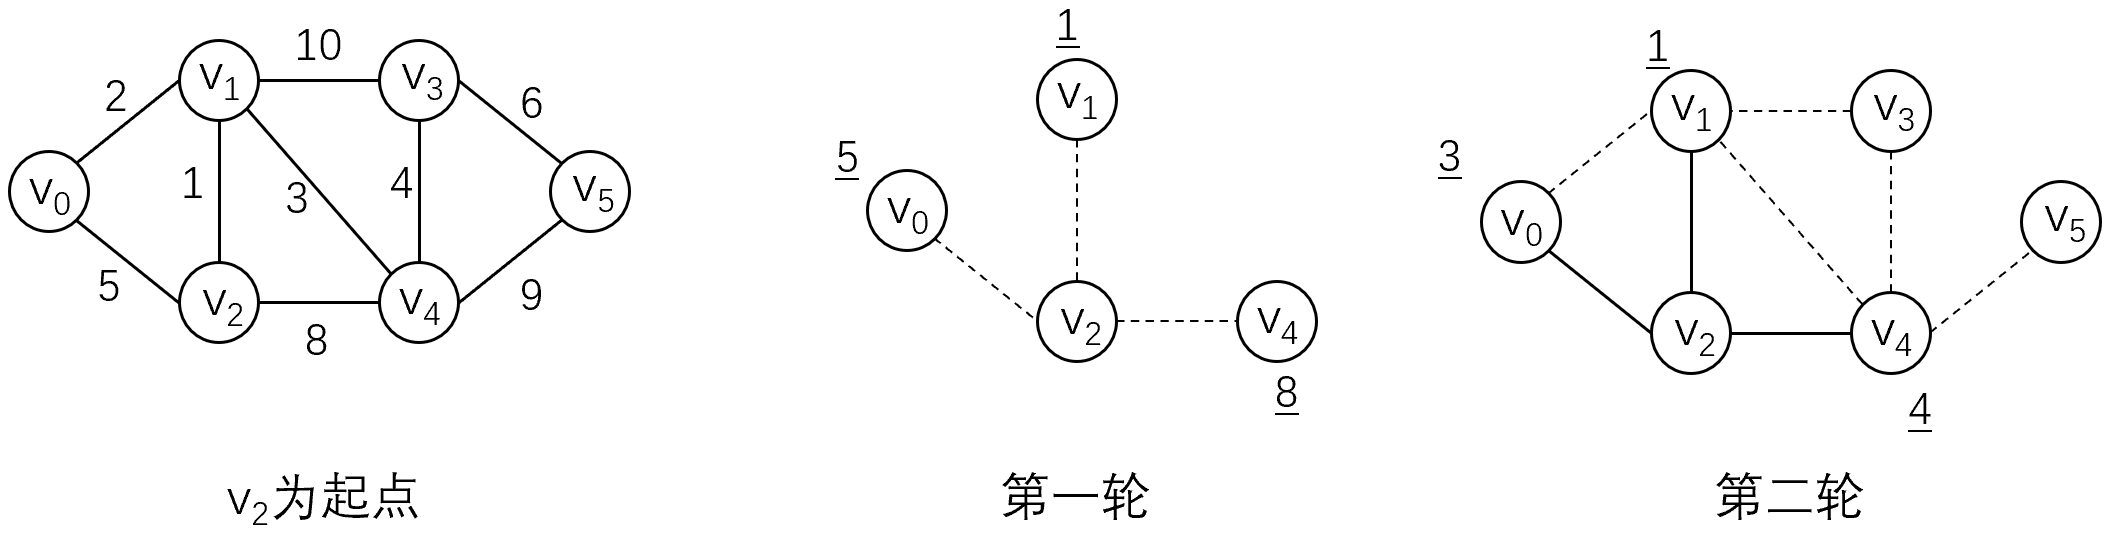
\includegraphics[width=0.85\textwidth]{assets/pics_and_ppts/ch5/22BellmanFord算法理解.png}
    \caption{}
    \label{fig:BellmanFord算法理解}
\end{figure}

$v_0$到$v_2$的最短
路径是$v_0 -> v_1 -> v_2$、$v_4$到$v_2$的最短路径是$v_4 -> v_1 -> v_2$，都是2条边的最短路径，因此第二轮操作之后就能考虑到这些路径，并且赋值给
cur\_mind[0]、cur\_mind[4]，之后绝对不会再改变。

Bellman-Ford 算法每完成一轮对所有边的松弛，就能够保证考虑到最多多一条边的路径，因此$N-1$轮之后，就能考虑到最多$N-1$条边的路径。而
如果源点可达范围不存在负权环，那么任意两个顶点之间的最短路径一定不包含重复顶点，路径最多$N-1$条边。

此外，如果完成 \(N-1\) 轮后，再对所有边进行一轮松弛，仍然能够更新某个顶点的距离，就说明存在从源点可达的负权环。若图存在从源点可达的负环，则显然在负环
中不断转圈可以让最短路径无限地小下去，直至负无穷。因此，通过以上手段Bellman-Ford算法可以在图不存在负环时给出正确解，并在图存在负环时给出“问题不可解”的结论。

Bellman-Ford 算法需要做约$N$轮操作，每轮操作需要遍历所有边，对于邻接矩阵存储的图，遍历所有边需要遍历邻接矩阵，时间为$O(N^2)$，而对于邻接表，遍历所有边
需要遍历邻接表，时间为$O(M)$。因此对于邻接矩阵存储的图，Bellman-Ford时间复杂度为$O(N^3)$，对于邻接表存储的图，Bellman-Ford的时间复杂度为$O(NM)$。

对于邻接表存储的图，Bellman-Ford算法的实现如下所示：
\begin{cppcode}
    struct AdjEdge {
        int u;
        int weight;
    };
    vector<AdjEdge> AdjList[N]; // 已存储图的邻接表
    const int inf = 0x3fffffff;
    int cur_mind[N];    // 已初始化为inf
    int Pre[N];     // 已初始化为-1
    bool BellmanFord(int s) {
        cur_mind[s] = 0;
        // 做N-1次
        for(int i=0; i<N-1; i++) {
            // 遍历所有边
            for(int v=0; v<N; v++) {
                // 与v邻接的所有边
                for(int k=0; k<AdjList[v].size(); k++) {
                    int u = AdjList[v][k].u;
                    int weight = AdjList[v][k].weight;
                    if(cur_mind[v] + weight < cur_mind[u]) {
                        cur_mind[u] = cur_mind[v] + weight;
                        Pre[u] = v;
                    }

                }
            }
        }

        // 再做一次，判断是否存在负环
        for(int v=0; v<N; v++) {
            for(int k=0; k<AdjList[v].size(); k++) {
                int u = AdjList[v][k].u;
                int weight = AdjList[v][k].weight;
                if(cur_mind[v] + weight < cur_mind[u]) {
                    return false;
                }

            }
        }
        return true;
    }
\end{cppcode}
当图存在负环时，Bellman-Ford算法返回false，表示存在负环，最短路径问题不可解。否则返回true，cur\_mind[]数组中存放的就是各顶点的最短路径。沿着Pre[]数组
往回追溯即可得到轨迹。对于邻接矩阵版本仅在于遍历边的方式不同，这里不再给出代码。

可以看到，与Dijkstra算法从源点出发，逐渐向外“扩散”地求解各个顶点的最短路径的策略不同，Bellman-Ford算法则是“放眼全局”，一步一步地让全局下的各个cur\_mind[]
慢慢向正确解“收拢”。\\

对于Bellman-Ford算法，我们自然会想到这样一个问题：我们每轮处理的时候，都需要遍历所有边，判断能否更新某个顶点的cur\_mind[]。但事实上，假设第$i-1$轮
仅有顶点v的cur\_mind[]发生了变化，那么第$i$轮其实我们没有必要遍历所有边，而是只遍历v的出边即可，因为只有距离发生了变化的顶点才可能继续影响其他顶点。这样，
仅处理距离发生了变化的边，就大大提高了算法的效率。因此对于上面的代码，在以下条件成立时：
\begin{cppcode}
    if(cur_mind[v] + weight < cur_mind[u]) {
        cur_mind[u] = cur_mind[v] + weight;
        Pre[u] = v;
    }
\end{cppcode}
说明u是一个距离发生了变化的顶点，我们将其放入队列中。

于是思路就是：最初将起点s放入队列，并在每次处理时，将那些距离发生了改变的顶点入队。当队列为空时，说明没有新的顶点距离发生改变，也就处理完了。但是这样做有两个新的问题：

（1）反复入队问题。

\begin{wrapfigure}{r}{0.27\textwidth}
    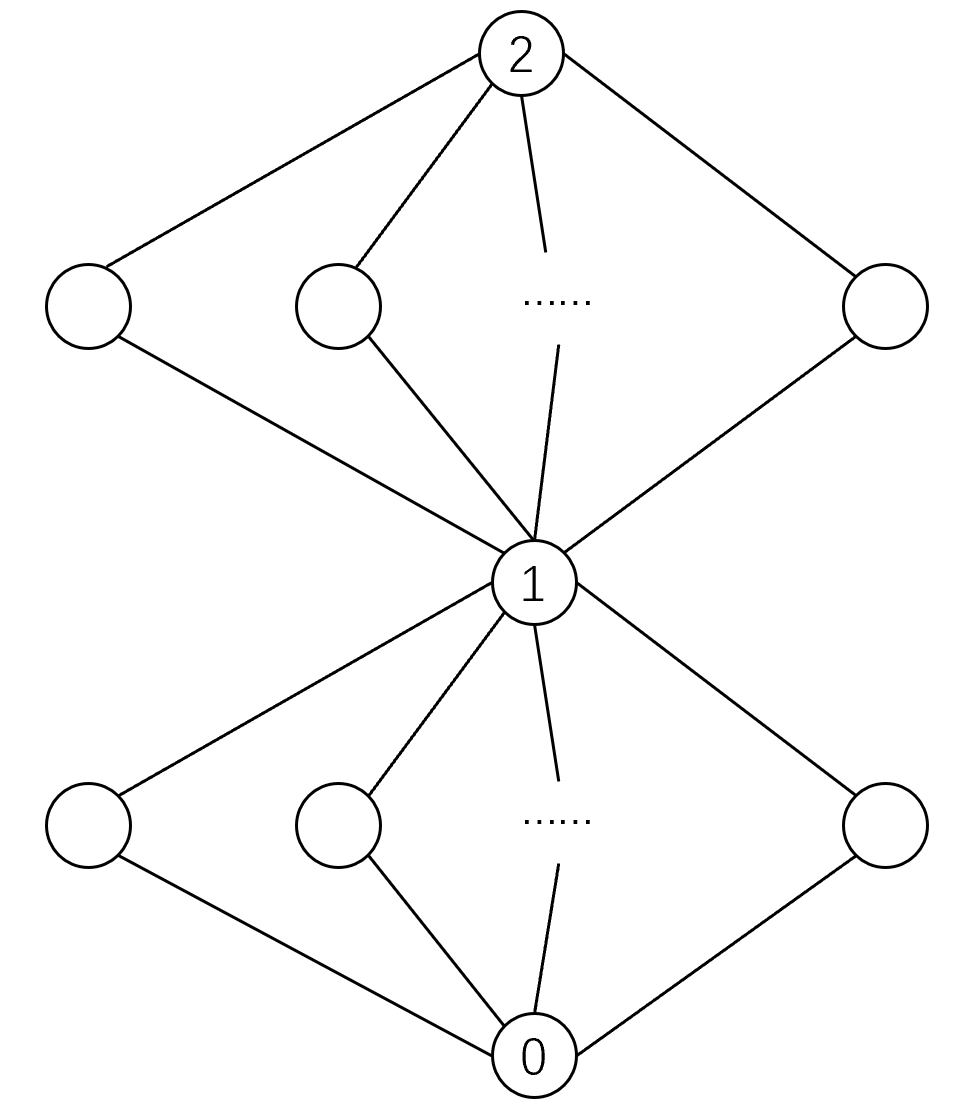
\includegraphics[width=0.35\textwidth]{assets/pics_and_ppts/ch5/23SPFA反复入队导致性能雪崩.png}
    \caption{反复入队问题}
    \label{fig:SPFA反复入队导致性能雪崩}
\end{wrapfigure}

如图\ref{fig:SPFA反复入队导致性能雪崩}所示，假设0为起点，向上松弛的若干顶点，将这些顶点入队后，
取出时，对每一个顶点的处理都可能将顶点1松弛一遍，如果每次都将1入队就造成了重复入队，会出现很多无意义的重复处理，继续向外传导，会造成指数级的性能灾难。因此要
解决这个问题，就需要引入一个数组in\_queue[N]，标识每一个顶点是否已经在队列中了，顶点此时不在队列中时才将它入队。



（2）负环判断问题。这种做法一直做到队列为空，若存在负环，则永远会有新的顶点距离变小，队列永远不会空。那怎么办？常见的做法是再记录一个数组
inq\_cnt[N]，标记每个顶点入队的次数。若某个顶点已经入队了超过$N-1$次（它的距离已经被更新过超过$N-1$次），说明存在负环，问题不可解。

于是我们可以给出这种优化的Bellman-Ford算法代码（邻接表版）如下所示：
\begin{cppcode}
    struct AdjEdge {
        int u;
        int weight;
    };
    vector<AdjEdge> AdjList[N]; // 已存储图的邻接表
    const int inf = 0x3fffffff;
    int cur_mind[N];    // 已初始化为inf
    int Pre[N];     // 已初始化为-1

    bool in_queue[N];   // 标记顶点是否当前在队列中，初始化为false
    int inq_cnt[N];         // 记录顶点入队次数，用于检测负权环，初始化为0
    bool SPFA(int s) {
        cur_mind[s] = 0;
        queue<int> q;
        q.push(s);
        in_queue[s] = true;

        while(!q.empty()) {
            int v = q.front();
            q.pop();
            
            // 弹出后，别忘了将标记改为 false，允许它以后再次入队
            in_queue[v] = false;

            // 遍历当前顶点的所有出边
            for(int j = 0; j < AdjList[v].size(); j++) {
                int u = AdjList[v][j].u;
                int weight = AdjList[v][j].weight;

                // 松弛操作
                if(cur_mind[v] + weight < cur_mind[u]) {
                    cur_mind[u] = cur_mind[v] + weight;
                    Pre[u] = v;

                    // 如果 u 不在队列中，将其压入队列
                    if(!in_queue[u]) {
                        q.push(u);
                        in_queue[u] = true;
                        inq_cnt[u]++; // 记录入队次数

                        // 如果某个顶点入队次数超过 N-1 次，说明存在负权环
                        if(inq_cnt[u] >= N) {
                            return false; 
                        }
                    }
                }
            }
        }

        return true; 
    }
\end{cppcode}

这种优化后的Bellman-Ford算法被称为\term{SPFA（Shortest Path Faster Algorithm）算法}。它的平均时间复杂度为O(kM)，k是每个顶点的
平均入队次数，而最坏时间复杂度为O(NM)。在大多数场景下SPFA算法性能要由于堆优化后的迪杰斯特拉算法，但对于极端情况，迪杰斯特拉算法
最差也能保证O((N+M)logN)的复杂度，而SPFA算法可能达到O(NM)。


\subsection{Floyd算法}
Floyd 算法（弗洛伊德算法），是一种用于求解图中所有顶点对之间最短路径的算法，即\term{全源最短路径}问题。。
Floyd算法的核心思想在于：对于任意三个顶点 \(i\)、\(j\)、\(k\)，我们都可以尝试：
\[
    d_{ij}=\min(d_{ij},d_{ik}+d_{kj})
\]
也就是说，我们原来知道的\(i\) 到 \(j\) 的最短距离是 \(d_{ij}\)，现在尝试让路径经过顶点 \(k\)，如果经过 \(k\) 的距离更短，就更新答案。

顶点到自身的距离初始化为$0$，存在直接边的顶点之间距离初始化为边权，不存在直接边的顶点之间距离初始化为正无穷。算法实现如下：
\begin{cppcode}
    const int inf = 0x3fffffff;
    int d[N][N];

    // 初始化距离矩阵
    for (int i = 0; i < N; i++) {
        for (int j = 0; j < N; j++) {
            d[i][j] = (i == j ? 0 : inf);
        }
    }

    // 根据图中的边更新距离矩阵
    // 假设存在一条从u到v、权重为w的边
    degree[u][v] = w;
    // ...

    // Floyd算法
    for (int k = 0; k < N; k++) {
        for (int i = 0; i < N; i++) {
            for (int j = 0; j < N; j++) {
                if (d[i][k] != inf &&
                    d[k][j] != inf) {
                    d[i][j] = min(
                        d[i][j],
                        d[i][k] + d[k][j]
                    );
                }
            }
        }
    }
\end{cppcode}
Floyd算法支持存在负权边的图，但要求不存在从源点可达的负权环。其时间复杂度为$O(N^3)$，空间复杂度为$O(N^2)$。






\chapter*{--- BONFIRE ENCOUNTERED ---}%%%%%%%%%%%%%%%%%%%%%%%%%%%%%%%%%%%%%%%%%%%%%%%%%%%%%%%%%%%%%%%%%%%%%%%%%%%%%%%%%%%%%%%%%%%%%%%%%%%%%%%%%%%%%%%%%%%%%%%%%%%%%%%%%%%%%%%%%%
火光闪烁中，你独自坐在营火旁。


\begin{exercise}
1. （某年408真题）使用迪杰斯特拉算法求下图中顶点1到其他各顶点之间的最短路径，则依次确定最短路径的目标定点是\underline{\hspace{1cm}}
\begin{center}
    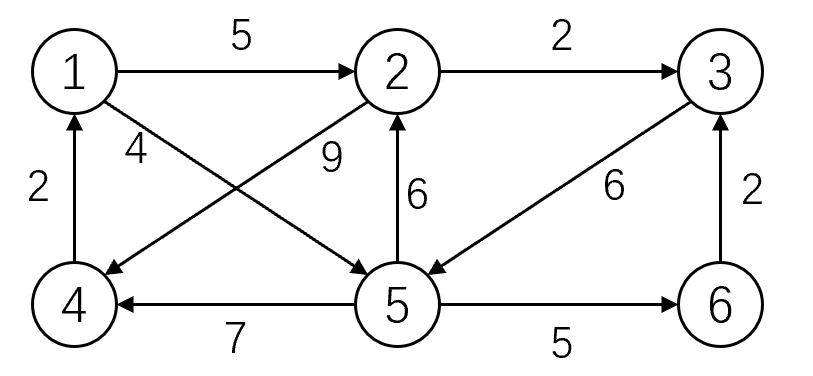
\includegraphics[width=0.40\textwidth]{assets/pics_and_ppts/ch5/习题09，16408最短路径的选点顺序.png}
\end{center}

\begin{tabular}{llll}
    A. 5,2,3,4,6 & B. 5,2,3,6,4 & C. 5,2,4,3,6 & D. 5,2,6,3,4
\end{tabular}

\vspace{\baselineskip}

2. （某年408真题）对下图所示的有向带权图，若采用迪杰斯特拉算法求源点a到其他各顶点的最短路径，则第一个确定全局最短路径的顶点是b，第二个确定全局最短路径
的顶点是c，后续的顶点依次是\underline{\hspace{1cm}}

\begin{center}
    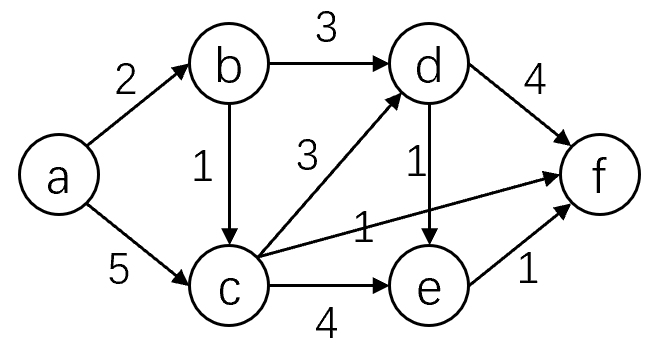
\includegraphics[width=0.34\textwidth]{assets/pics_and_ppts/ch5/习题10，12408最短路径选点顺序.png}
\end{center}

\begin{tabular}{llll}
    A. d,e,f & B. e,d,f & C. f,d,e & D. f,e,d
\end{tabular}

\vspace{\baselineskip}

3. （某年408真题）使用迪杰斯特拉算法求下图中从顶点1到其余各顶点的最短路径，将当前找到的从顶点1到顶点2，3，4，5的最短路径
保存在数组dist[]中，则依次求出两个顶点（不包括源点1）的最短路径后，dist中的内容更新为\underline{\hspace{1cm}}

\begin{center}
    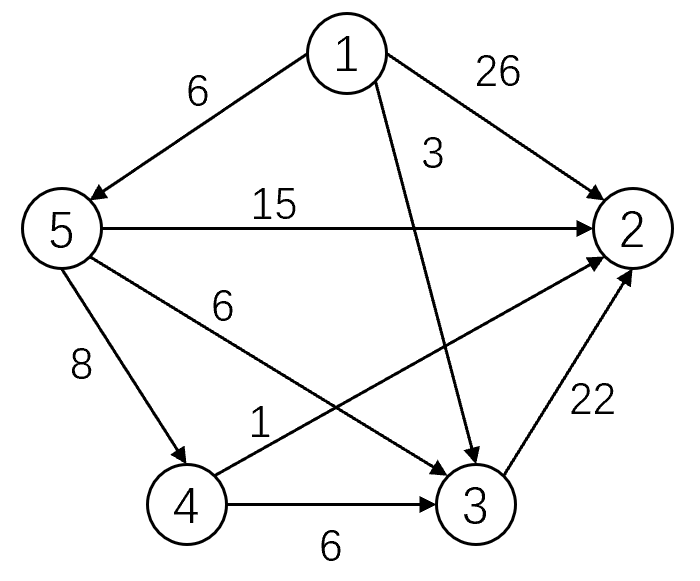
\includegraphics[width=0.33\textwidth]{assets/pics_and_ppts/ch5/习题11，21408迪杰斯特拉dist内容.png}
\end{center}

\begin{tabular}{llll}
    A. 26,3,14,6 & B. 25,3,14,6 & C. 21,3,14,6 & D. 15,3,14,6
\end{tabular}

\vspace{\baselineskip}

4. 请你说明：迪杰斯特拉算法、Bellman-Ford算法以及SPFA算法应对以下情况的图时会怎样？\\[0.5em]
a）存在从源点可达的负环；\\
b）不存在从源点可达的负环，但存在从源点可达的负权边；\\

维火女被邪恶的恶魔、大陆守护神的孪生兄弟LoopCore抓了起来，并关在了监牢的某个牢房里。监牢可以被建模为一个图$G=(V,E)$，顶点表示牢房。

已知该监牢有 $N$ 个牢房，编号为 0 到 $N-1$，牢房之间均存在双向通路，用邻接表存储图模型。你毫不犹豫地动身前往牢房营救维火女，但你破门而入后意外地被魔法传送进了牢房s。\\

5. 已知每个牢房（顶点）的数据类型为char：维火女所在的牢房为\textquotesingle T\textquotesingle，其余牢房均为\textquotesingle F\textquotesingle。
给出在每两个牢房之间移动所需要花费的时间time\_cost（非负），请你计算从s出发，到达维火女的房间所需要的最短时间是多少，若无法到达，返回-1。

\begin{cppcode}
    // N 已定义
    struct AdjEdge {
        int u;          // 顶点编号
        int time_cost;  // 花费时间（边权）
    };
    vector<AdjEdge> AdjList[N];    // 已存储邻接表信息 
    char ver_info[N];   // 已存储顶点信息
    // 返回以s为起点到达维火女的房间需要花费的最短时间
    int MinTime(int s) {
        
    }
\end{cppcode}

\vspace{\baselineskip}

6. 在{\color{red}上题}条件下，假设你在任何两个房间移动时需要和敌人战斗，此时邻接边（AdjEdge）使用如下结构定义：
\begin{cppcode}
    struct AdjEdge {
        int u;              
        int time_cost;      // 花费时间
        int energy_cost;    // 和敌人战斗需要消耗的能量值
    };
\end{cppcode}
保证所有边的time\_cost和energy\_cost均非负。你决定选择所有路线中，消耗时间最少的路线去营救维火女。若有多条路线消耗时间相等，你将选择其中
消耗能量最少的一条路线。

编写一个函数，返回你所选择的路线所消耗的能量值。若无法到达，返回-1。\\

% *7. 在{\color{red}上题}条件下，若你的初始能量值为$e_1$，并且在你到达维火女的房间后，至少还剩有$e_2$的能量值的前提下，才能带她一起离开监牢。
% 现要求你找到她后，必须能够带她离开监牢。在此前提下，你将选择时间最短的一条路线，若有多条路线，你将选择消耗能量最少的路线。请返回在此路线下你
% 到达维火女的房间时剩余的能量值。

% \begin{cppcode}
%     // N 已定义
%     struct AdjEdge {
%         int u;              
%         int time_cost;      // 花费时间
%         int energy_cost;    // 和敌人战斗需要消耗的能量值
%     };
%     vector<AdjEdge> AdjList[N];    // 已存储邻接表信息 
%     char ver_info[N];   // 已存储顶点信息
%     // 返回以s为起点到达维火女的房间需要花费的最短时间
%     int RemainingEnergy(int s, int e1, int e2) {
        
%     }
% \end{cppcode}



\end{exercise}
\clearpage

\begin{exerciseanswer}
1. 选B。每一步所选的点，及选完该点后所有点的当前已知最短路径cur\_mind[]如下图所示（带下划线的数字表示该顶点的cur\_mind[]）。
\begin{center}
    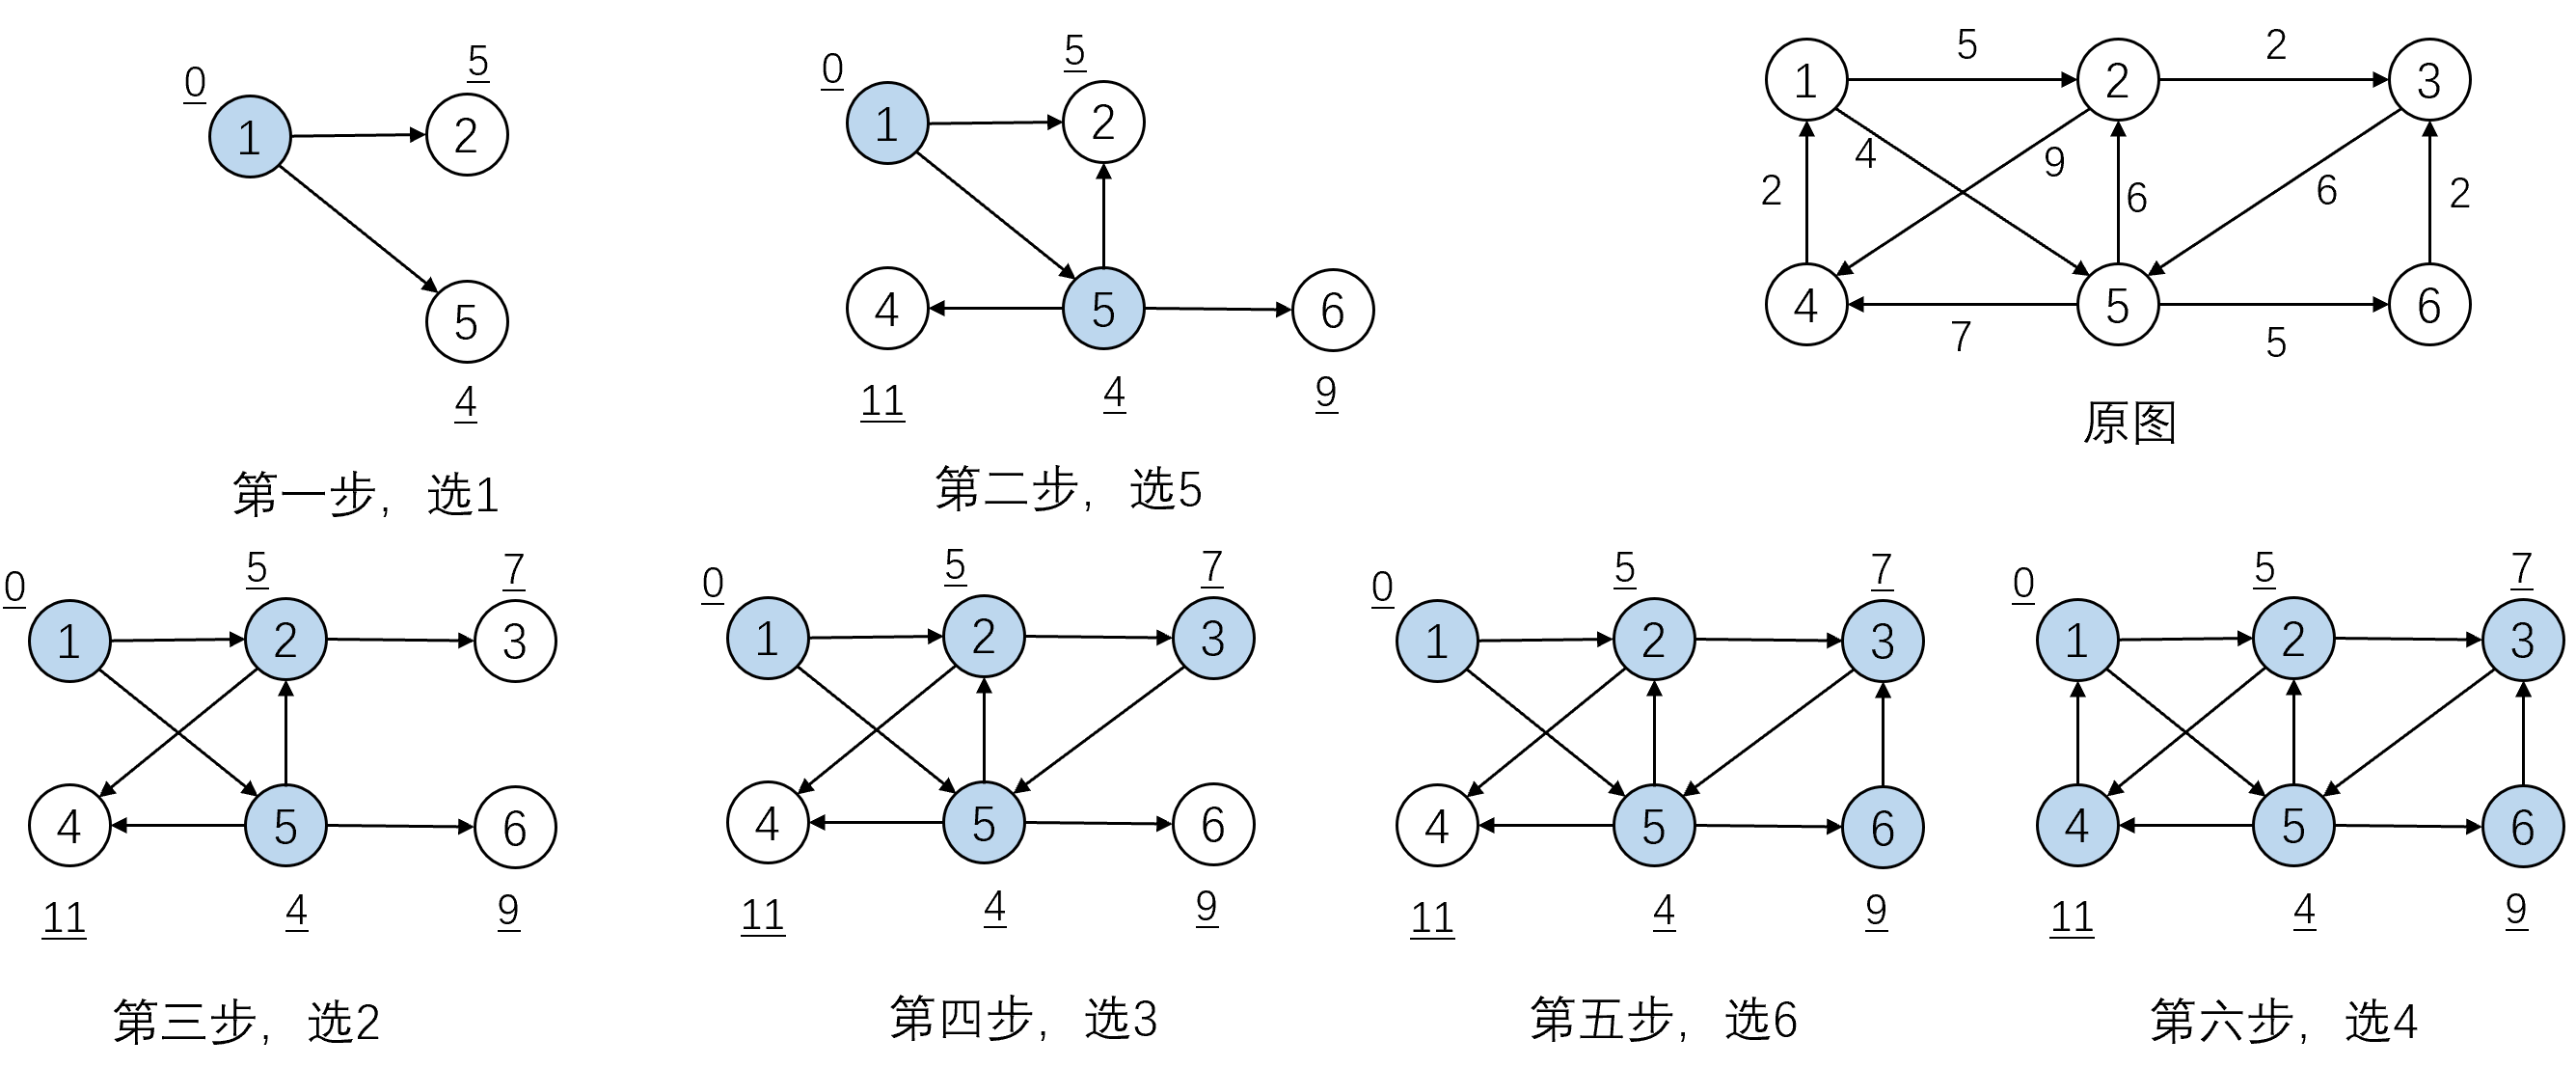
\includegraphics[width=1.02\textwidth]{assets/pics_and_ppts/ch5/习题09，16408最短路径的选点顺序答案图.png}
\end{center}
于是选点顺序是1,5,2,3,6,4，选B。\\

2. 选C。需要注意c到f是有一条边的，别看漏了就行。\\

3. 选C。求解前两个顶点（不包括源点）的最短路径过程如下所示。
\begin{center}
    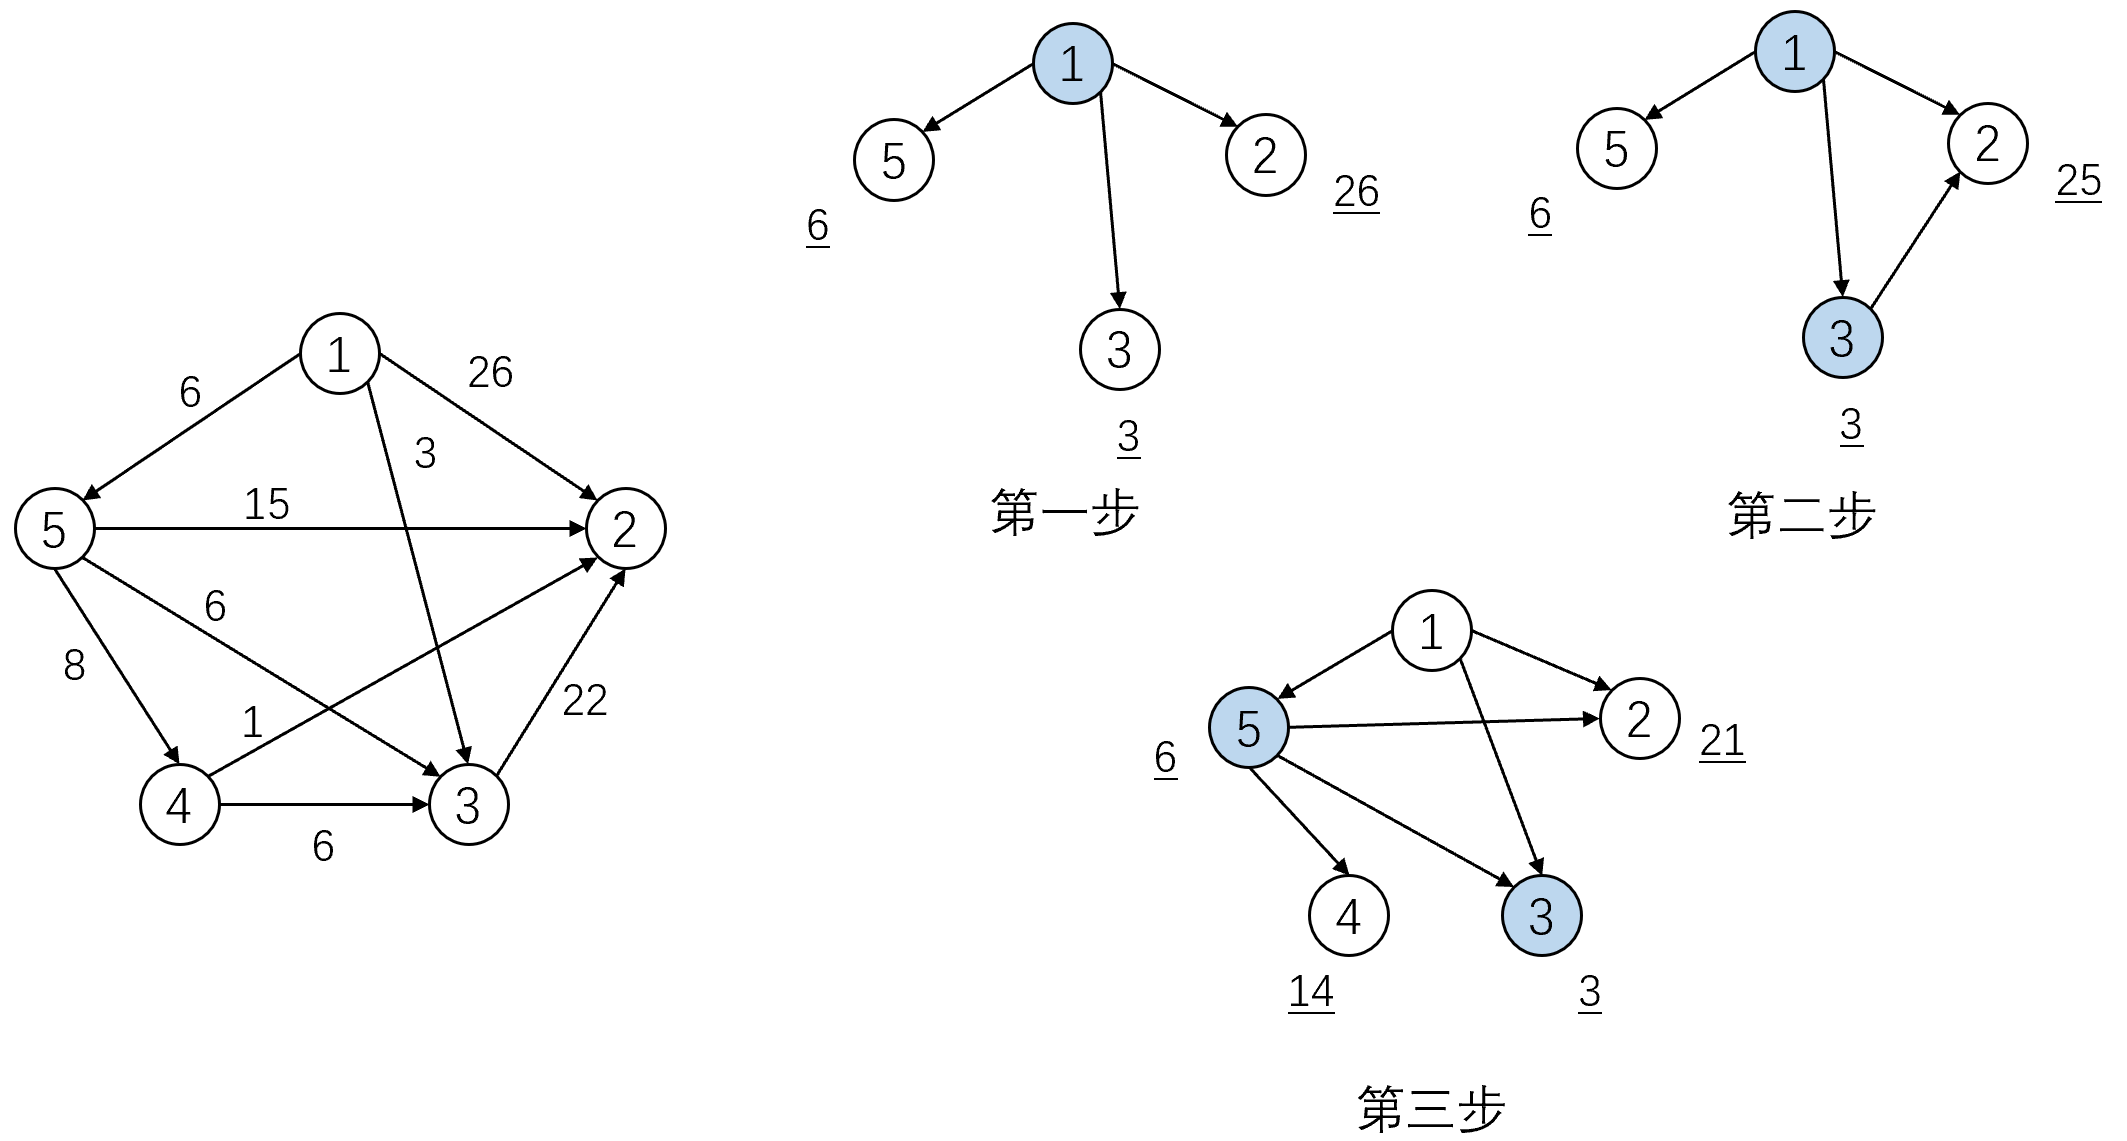
\includegraphics[width=0.90\textwidth]{assets/pics_and_ppts/ch5/习题11，21408迪杰斯特拉dist内容答案图.png}
\end{center}

\vspace{\baselineskip}

4. a）若存在从源点可达的负环，则源点s与任何一个顶点v的最短路径，都可以通过“先走到负环，然后一直绕圈，再走到v”的方式，将最短路径“刷到负无穷”，因此若图中
存在源点可达的负环，通常认为最短路径问题不可解，或者为负无穷；而Bellman-Ford算法可以在图存在负环时给出“不可解”的结论，Dijkstra算法则难以做到这一点。

b）若存在源点可达的负权边，那么迪杰斯特拉算法将失效，求解出可能错误的最短路径；而Bellman-Ford及SPFA算法可以应对存在负权边的图，给出正确的最短路径。

三种算法总结如下：\\

\begin{tabular}{|c|c|c|c|}
    \hline
    \textbf{图的特点} &	\textbf{Dijkstra} &	\textbf{Bellman-Ford} &	\textbf{SPFA}\\
    \hline
    所有边权非负 &	可以 & 可以 & 可以\\
    \hline
    存在负权边，无可达负环 & 不保证正确 & 可以 & 可以 \\
    \hline
    存在可达负权环 & 不保证正确，无法可靠检测 & 可以检测 & 可以检测\\
    \hline
\end{tabular}

\vspace{\baselineskip}

5. 本题意在给大家练习求解最短路径的迪杰斯特拉算法、SPFA算法的代码。显然，我们使用算法求出各顶点的最短路径，返回维火女所在顶点的最短路径即可。
使用迪杰斯特拉算法求解的代码如下：
\begin{cppcode}
    // N 已定义
    struct AdjEdge {
        int u;          // 顶点编号
        int time_cost;  // 花费时间（边权）
    };
    vector<AdjEdge> AdjList[N];    // 已存储邻接表信息 
    char ver_info[N];   // 已存储顶点信息
    // 返回以s为起点到达维火女的房间需要花费的最短时间
    int MinTime(int s) {
        const int inf = 0x3fffffff;
        int cur_mind[N];
        bool solved[N];
        // 记录维火女所在的牢房编号firekeeper_idx，函数最后返回cur_mind[firekeeper_idx]。
        int firekeeper_idx = -1;
        
        // 初始化的过程顺便找一下维火女在哪
        for(int i=0; i<N; i++) {
            cur_mind[i] = inf;
            solved[i] = false;
            if(ver_info[i] == 'T') {
                firekeeper_idx = i;
            }
        }
        cur_mind[s] = 0;

        for(int i=0; i<N-1; i++) {
            // 从尚未求解的顶点中选出一个cur_mind[]最小的顶点v
            int min_curmind = inf;
            int v = -1;
            for(int j=0; j<N; j++) {
                if(cur_mind[j] < min_curmind && !solved[j]) {
                    v = j;
                    min_curmind = cur_mind[j];
                }
            }

            if(v == -1) {
                break;
            }
            solved[v] = true;
            // 已经计算出维火女了，就别再计算其他的了，赶紧去救她吧！
            if(v == firekeeper_idx) {
                return cur_mind[v];
            }

            for(int j=0; j<AdjList[v].size(); j++) {
                int u = AdjList[v][j].u;
                int time_cost = AdjList[v][j].time_cost;
                if(cur_mind[v] + time_cost < cur_mind[u]) {
                    cur_mind[u] = cur_mind[v] + time_cost;
                }
            }
            
        }
        return cur_mind[firekeeper_idx] == inf? -1 : cur_mind[firekeeper_idx];
    }
\end{cppcode}

使用SPFA算法求解的代码如下：
\begin{cppcode}
    // N 已定义
    struct AdjEdge {
        int u;          // 顶点编号
        int time_cost;  // 花费时间（边权）
    };
    vector<AdjEdge> AdjList[N];    // 已存储邻接表信息 
    char ver_info[N];   // 已存储顶点信息
    // 返回以s为起点到达维火女的房间需要花费的最短时间
    int MinTime(int s) {
        const int inf = 0x3fffffff;
        int cur_mind[N];
        bool in_queue[N];
        /* 该场景明确图中无负边，因此无需进行负环
        检测，也就不需要inq_cnt[]数组，但这里还是
        以注释给出，帮助大家再次复习若需要检测负环
        时，代码该怎么写。 */
        // int inq_cnt[N];  
        int firekeeper_idx = -1;
        for(int i=0; i<N; i++) {
            cur_mind[i] = inf;
            in_queue[i] = false;
            // inq_cnt[i] = 0;
            if(ver_info[i] == 'T') {
                firekeeper_idx = i;
            }
        }
        cur_mind[s] = 0;
        queue<int> q;
        q.push(s);
        in_queue[s] = true;
        while(!q.empty()) {
            int v = q.front();
            q.pop();
            in_queue[v] = false;
            for(int i=0; i<AdjList[v].size(); i++) {
                int u = AdjList[v][i].u; 
                int time_cost = AdjList[v][i].time_cost;
                if(cur_mind[v] + time_cost < cur_mind[u]) {
                    cur_mind[u] = cur_mind[v] + time_cost;
                    if(!in_queue[u]) {
                        in_queue[u] = true;
                        q.push(u);
                        // inq_cnt[u] += 1;
                    }

                    // 若可能存在负环，在此处进行负环判断
                    
                }
            }
        }
        return cur_mind[firekeeper_idx] == inf ? -1 : cur_mind[firekeeper_idx];
    }
\end{cppcode}

\vspace{\baselineskip}

6. 

\begin{wrapfigure}{r}{0.22\textwidth}  
    \centering
    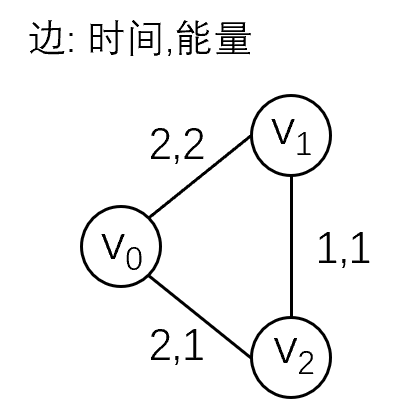
\includegraphics[width=0.80\linewidth]{assets/pics_and_ppts/ch5/习题12营救维火女最短时间、最小能量答案图.png}
\end{wrapfigure}

若使用迪杰斯特拉算法，就要同时记录每个点的当前已知最短时间及对应最短时间路径的最小能量消耗：cur\_mint[i]为j表示顶点i到s的最短时间为j，并且cur\_mine[i]
为k表示顶点i到s的最短时间路径下，最小消耗为k。

而且每次“选点”时，就不能只选择时间花费最小的，而是要选的时间花费最小的条件下，能量消耗最小的那个点。如图，
以$v_0$为起点，若直接选择了$v_1$，则会得到错误答案。在更新时类似，当时间更短，或时间相等但能量消耗更少时更新即可。代码如下：

\begin{cppcodeHighlight}[11-12,17-18,29-30,32-39,53-59]
    // N 已定义
    struct AdjEdge {
        int u;          
        int time_cost;      // 花费时间
        int energy_cost;    // 和敌人战斗需要消耗的能量值
    };
    vector<AdjEdge> AdjList[N];    // 已存储邻接表信息 
    char ver_info[N];   // 已存储顶点信息
    // 返回以s为起点到达维火女的房间花费时间最短的路径中，消耗能量最少的那条路径所消耗的能量值
    int MinEnergyCost(int s) {
        int cur_mint[N];    // 当前已知的各顶点最短时间
        int cur_mine[N];    // 对应最短时间路径中的最小能量消耗
        bool solved[N];
        const int inf = 0x3fffffff;
        int firekeeper_idx = -1;
        for(int i=0; i<N; i++) {
            cur_mint[i] = inf;
            cur_mine[i] = inf;
            solved[i] = false;
            if(ver_info[i] == 'T') {
                firekeeper_idx = i;
            }
        }

        cur_mint[s] = 0;
        cur_mine[s] = 0;
        
        for(int i=0; i<N-1; i++) {
            int min_timecost = inf;
            int min_energycost = inf;
            int v = -1;
            for(int j=0; j<N; j++) {
                if(!solved[j] && (cur_mint[j] < min_timecost || 
                    cur_mint[j] == min_timecost && cur_mine[j] < min_energycost) 
                ) {
                    min_timecost = cur_mint[j];
                    min_energycost = cur_mine[j];
                    v = j;
                }
            }

            if(v == -1) {
                break;
            }
            solved[v] = true;
            if(v == firekeeper_idx) {
                break;
            }
            for(int j=0; j<AdjList[v].size(); j++) {
                int u = AdjList[v][j].u;
                int time_cost = AdjList[v][j].time_cost;
                int energy_cost = AdjList[v][j].energy_cost;
                if(cur_mint[v] + time_cost < cur_mint[u]) {
                    cur_mint[u] = cur_mint[v] + time_cost;
                    cur_mine[u] = cur_mine[v] + energy_cost;
                }
                else if(cur_mint[v] + time_cost == cur_mint[u] && cur_mine[v] + energy_cost < cur_mine[u]) {
                    cur_mine[u] = cur_mine[v] + energy_cost;
                }
            }
        }
        return cur_mine[firekeeper_idx] == inf ? -1 : cur_mine[firekeeper_idx];
    }
\end{cppcodeHighlight}
事实上本题可以从另一个角度去理解：有些时候我们可能在求时间最短的最短路径，有些时候求路程最短，有些时候求花费最少......，时间、路程、花费的大小比较规则就是比数值。

而本题“时间”和“能量”共同组成了某个东西，拟叫它“代价”好了，那么本题其实就是在求“代价”最短的最短路径。只不过“代价”有着不太一样的大小比较规则：对于两个表示
“代价”的变量a和b，

1）a“小于”b定义为：a的时间比b小，或a与b时间相等并且a的能量比b小；

2）a“等于”b定义为：a与b的时间、能量完全相等；

3）a“大于”b定义为：a的时间比b大，或a与b时间相等并且a的能量比b大；

因此，我们在每次“选点”时，就像要以时间、路程、花费等为标尺选出最小的一样，本题我们就是在选出“代价”最小的；在更新时，是在比较“代价”的大小，若以v为中介，
能够使得u的“代价”更小，则更新u。这也从另一个角度理解了以上代码实现。

同时，通过C++的运算符重载功能，我们可以对这种结构体的大小比较进行定义：
\begin{cppcode}
    struct cost {
        int time ;
        int energy;
        // 定义cost类型对象的“<”比较规则
        bool operator < (const cost& other) const {
            return this->time < other.time ||
                (this->time == other.time && this->energy < other.energy);
        }

        // 定义两个代价相加规则
        cost operator + (const cost& other) const {
            cost ret;
            ret.time = this->time + other.time;
            ret.energy = this->energy + other.energy;
            return ret;
        }
    };
    cost cur_minc[N];   // 这一个数组就包含了cur_mint和cur_mine的功能
\end{cppcode}
然后每次“选点”时：
\begin{cppcode}
    cost min_cost;
    min_cost.time = inf;
    min_cost.energy = inf;
    int v = -1;
    for(int j=0; j<N; j++) {
        if(!solved[j] && cur_minc[j] < min_cost ) {
            min_cost = cur_minc[j];
            v = j;
        }
    }
    ...
\end{cppcode}
更新时：
\begin{cppcode}
    for(int j=0; j<AdjList[v].size(); j++) {
        int u = AdjList[v][j].u;
        cost c;
        c.time = AdjList[v][j].time_cost;
        c.energy = AdjList[v][j].energy_cost;
        if(cur_minc[v] + c < cur_minc[u]) {
            cur_minc[u] = cur_minc[v] + c;
        }
    }
\end{cppcode}
这种运算符重载规则，可以在我们使用C++标准库提供的排序函数std::sort()时来自定义一些排序规则，我们将在\ref{minisec:Kruskal算法实现}节（
第\pageref{minisec:Kruskal算法实现}页）中看到。



\end{exerciseanswer}%%%%%%%%%%%%%%%%%%%%%%%%%%%%%%%%%%%%%%%%%%%%%%%%%%%%%%%%%%%%%%%%%%%%%%%%%%%%%%%%%%%%%%%%%%%%%%%%%%%%%%%%%%%%%%%%%%%%%%%%%%%%%%%%%%%%%%%%%